%% LyX 2.1.4 created this file.  For more info, see http://www.lyx.org/.
%% Do not edit unless you really know what you are doing.
\documentclass[a4paper,twoside,english]{report}
\usepackage[utf8]{inputenc}
\setcounter{secnumdepth}{3}
\usepackage{babel}
\usepackage{array}
\usepackage{booktabs}
\usepackage{textcomp}
\usepackage{url}
\usepackage{multirow}
\usepackage{amsmath}
\usepackage{graphicx}
\usepackage{nomencl}
% the following is useful when we have the old nomencl.sty package
\providecommand{\printnomenclature}{\printglossary}
\providecommand{\makenomenclature}{\makeglossary}
\makenomenclature
\usepackage[unicode=true,
 bookmarks=false,
 breaklinks=false,pdfborder={0 0 1},backref=section,colorlinks=false]
 {hyperref}

\makeatletter

%%%%%%%%%%%%%%%%%%%%%%%%%%%%%% LyX specific LaTeX commands.
\pdfpageheight\paperheight
\pdfpagewidth\paperwidth

\newcommand{\noun}[1]{\textsc{#1}}
%% Because html converters don't know tabularnewline
\providecommand{\tabularnewline}{\\}
%% A simple dot to overcome graphicx limitations
\newcommand{\lyxdot}{.}


%%%%%%%%%%%%%%%%%%%%%%%%%%%%%% User specified LaTeX commands.


\usepackage[colorinlistoftodos]{todonotes}
\usepackage{placeins}
\usepackage{parskip}

\usepackage{subcaption}
\usepackage{tikz}


% for tables: \toprule, \midrule, \bottomrule
\usepackage{array}% for tables: \bfseries

\makeatother

\begin{document}
\thispagestyle{empty}

\vspace*{3cm}


\begin{center}
{\LARGE{}Marine cybernetics}
\par\end{center}{\LARGE \par}

\begin{center}
{\LARGE{}laboratory handbook }
\par\end{center}{\LARGE \par}

\begin{flushleft}
\vfill{}

\par\end{flushleft}

\begin{flushleft}

\includegraphics[scale=0.6]{NTNU_logo}
\par\end{flushleft}

Faculty of Engineering Science and Technology\\
Department of Marine Technology

\clearpage{}\thispagestyle{empty}\vspace*{3cm}


\clearpage{}

\pagenumbering{roman}\setcounter{page}{1}

\vspace*{3cm}



\section*{Introduction}

This handbook is a comprehensive reference for the marine hardware-in-the-loop
(HIL) and marine cybernetics laboratories. The laboratories are used
in teaching and research on development and real-time testing of marine
control systems.


\section*{Structure}

Part \ref{part: Theory} explains the concepts and motivations for
real-time and HIL testing.

Part \ref{part: Laboratory equipment} describes the laboratory facilities
and equipment. A general overview of hardware and software.

Part \ref{part: Laboratory user guide} is a user guide intended for
students of the course. Step-by-step instructions for development
and deployment of programs to the real-time controller are given.
Lower level details, intended for laboratory assistants and customized
use, are given in Part \ref{part: Equipment setup and configuration}.

Part \ref{part: Lab exercises} holds the exercise texts for TMR4243
Marine Control Systems II.

\newpage{}\tableofcontents{}

\newpage{}\settowidth{\nomlabelwidth}{FPGA}
\printnomenclature{}

\nomenclature{BT}{bow thruster}

\nomenclature{cRIO}{compact reconfigurable input/output real-time embedded industrial controller by National Instruments}

\nomenclature{CSE1}{Cybership Enterprise 1}

\nomenclature{CSS}{Cybership Saucer}

\nomenclature{DP}{dynamic positioning}

\nomenclature{ESC}{electronic speed controller}

\nomenclature{FPGA}{field-programmable gate array}

\nomenclature{HIL}{hardware-in-the-loop}

\nomenclature{MC}{marine cybernetics}

\nomenclature{PWM}{pulse-width modulation}

\nomenclature{RPi}{Raspberry Pi single-board computer}

\nomenclature{VSP}{Voith Schneider propeller}



\newpage{}

\pagenumbering{arabic}


\part{\label{part: Theory}Theory}


\chapter{Realtime}

Real-time testing involves using a real-time OS as part of a test
system. The most common requirements driving the need for a real-time
test system are to achieve greater reliability and performance than
is possible using a general-purpose OS. 

http://www.ni.com/white-paper/3938/en/

http://www.ni.com/white-paper/14238/en/

http://www.ni.com/white-paper/13068/en/
\begin{itemize}
\item Forklaring av hva realtime betyr i HW og SW
\end{itemize}

\chapter{HIL}

In general, Hardware-In-the-Loop simulation is a method that can be
used to test complex real-time control and monitoring systems. Such
systems are becoming more complex and rely on more advanced integrated
functionality of software-based real-time functions, and many separately
designed control and monitoring systems need to cooperate on performing
common tasks. Consequently, the control system software code becomes
more complex, and may be hard to verify by running regular software
simulations. With testing by HIL simulation, the control system is
run on its intended hardware, but instead of controlling the real
process, it is controlling a simulated process in a simulated environment.
The control and monitoring system will, however, see no difference
between the real process and the simulated process.

Through HIL testing, the Marine HIL-Lab aims for by students and researchers
to qualify their experimental setups in other laboratories before
their assigned laboratory time is started. This will aid in making
experimental work more efficient by reducing debugging time, improve
tuning of parameters and test scenarios, and thereby maximizing the
outcome of the experimental work.

Smogeli, Fremtidens verifikasjon av kontrollsystemer for Skip og offshorefartøy

DNV, Hardware in the Loop Testing (HIL)

Johansen, Sørensen, Experiences with HIL Simulator Testing of Power
Management Systems

Smogeli, Introduction to third- party HIL testing

Johansen, Fossen, Vik, Hardware-in-the-loop Testing of DP systems

Pivano, Experiences from seven years of DP software testing

DNV, Rules for Classification of Ships (Part 6, Ch 22)

Ambrosovskaya, Approach for Advanced Testing of DP Control System

Selvam, System Verification Helps Validate Complex Integrated Systems

A. Veksler prøveforelesning:
\begin{itemize}
\item Increased complexity marine vessels increases the need for testing
and verification.
\item A reasonably new approach to this is Hardware-In-the-Loop testing,
or HIL.
\item Widely used in the automotive industry
\item Can be seen as something in between simulation testing and full scale
testing

\begin{itemize}
\item More realistic than a simulation, less realistic than a full-scale
testing
\item Mathematical models of the systems that are not included as hardware.
\end{itemize}
\item A real-time simulator, constructed by hardware and software, that
is

\begin{itemize}
\item configured for the control system under consideration
\item embedded in external hardware
\item and interfaced to the target system or component through appropriate
I/O 
\end{itemize}
\item Advantages:

\begin{itemize}
\item Another layer of independent verification
\item Allows testing emergency procedures that would be too dangerous on
a real vessel
\end{itemize}
\item Disadvantages:

\begin{itemize}
\item Initial investment to set up a HIL simulator for a particular system.
The resources could be spent on simulation testing or full scale testing.
\item Supplements, but does not replace, proper software design techniques

\begin{itemize}
\item As with all software testing, it typically executes only a fraction
of the control system code. 
\end{itemize}
\end{itemize}
\end{itemize}
Asgeir
\begin{itemize}
\item HIL testing is accomplished by connecting a simulation PC in the system’s
communication network.
\item Inputs to the equipment under test are simulated.
\item The controllers respond as they would in a dynamic environment.
\item Simulator responds to output from the controllers as the dynamic system
would
\item Software (core SW and/or configuration) errors are exposed.
\end{itemize}

\chapter{Real-time computing}


\section{SIL}


\section{Model-in-the-loop}


\subsection{Hybrid simulation}

Another advantage of HIL testing is that scenarios that may be difficult
to test experimentally (either due to the risk involved in the test,
due to the need for a special state of the environment, or due to
inadequate experimental facilities), can be tested thoroughly, without
risk, if sufficient high-fidelity simulation software exists. This
also makes it possible to use the Marine HIL-Lab for hybrid experimental
test setups, where part of the experimental setup is real and part
is simulated, and these parts are interconnected through real-time
interfaces such as sensors, communications, and actuators.



\clearpage{}


\part{\label{part: Laboratory equipment}Laboratory descriptions}


\chapter{\label{sec: Marine HIL simulation laboratory}Marine HIL simulation
laboratory}

\begin{figure}
\centering 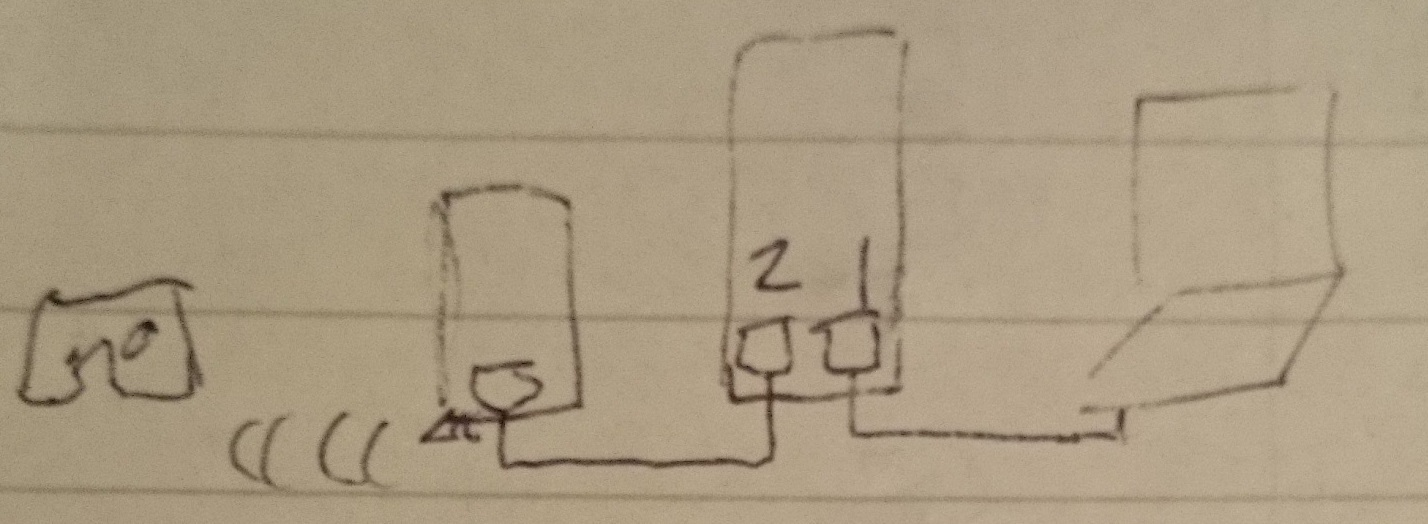
\includegraphics[width=0.95\textwidth]{setupHIL} \caption{\label{fig: HIL setup}HIL setup}
\end{figure}


The laboratory is suitable for implementation, qualification and comprehensive
testing of
\begin{itemize}
\item marine control algorithms
\item communication interfaces,
\item human-machine interfaces,
\item experimental test scenarios, and
\item experimental setups before proceeding to other laboratories (such
as model scale testing).
\end{itemize}

\section{Equipment}

The laboratory consists of three equivalent portable setups, as illustrated
in Figure \ref{fig: HIL setup}, each including 
\begin{itemize}
\item Sony Sixaxis wireless gamepad for PlayStation 3,
\item Raspberry Pi (RPi) with Bluetooth dongle,
\item National Instruments (NI) cRIO-9024 control and acquisition device,
and
\item Dell Latitude E6440 laptop.
\end{itemize}

\subsection{Hardware}


\subsubsection{Sixaxis wireless gamepad}

\begin{table}
\centering{}%
\begin{tabular}{cl}
\hline 
2 & analog joysticks\tabularnewline
1 & pressure-sensitive directional pad\tabularnewline
2 & analog triggers (L2, R2)\tabularnewline
6 & pressure-sensitive buttons (
\includegraphics[scale=0.4]{sixaxis_triangle},

\includegraphics[scale=0.4]{sixaxis_circle}, 
\includegraphics[scale=0.4]{sixaxis_cross},

\includegraphics[scale=0.4]{sixaxis_square}, L1, R1)\tabularnewline
5 & digital buttons (PS, L3, R3, Start, Select)\tabularnewline
 & motion sensing (6 degrees of freedom)\tabularnewline
\hline 
\end{tabular}\caption{\label{tab: sixaxis input}Sixaxis input}
\end{table}


The Sixaxis is a widespread gamepad. It transmits a broad range of
input, listed in Table \ref{tab: sixaxis input}, and is suitable
for human operator input. The device communicates over Bluetooth.


\subsubsection{Raspberry Pi}

The RPi is a credit card-sized single-board computer including Ethernet
and two USB connections. In the HIL laboratory setup, the unit is
merely used to transmit the Sixaxis' data to the cRIO\footnote{The cRIO USB port only supports common USB mass-storage devices, thus
a Bluetooth dongle cannot be connected directly.}.


\subsubsection{cRIO-9024}

The cRIO is a compact reconfigurable input/output embedded real-time
control and acquisition device, including two Ethernet ports. The
unit also holds a field-programmable gate array (FPGA) chassis. In
the HIL laboratory setup, an analog input module (NI 9215) and a digital
output module (NI 9474) are mounted on this chassis.


\subsubsection{Laptop}

A generic personal computer is used to configure and upload applications
to the cRIO. The same computer is used for graphical user interfacing
during simulations.


\subsection{Software}


\subsubsection{Laptop}

The main software used for the HIL laboratory are:
\begin{description}
\item [{MathWorks~Simulink}] graphical programming environment used for
implementation and compilation of dynamic systems simulation models
and control algorithms.
\item [{National~Instruments~VeriStand}] real-time testing environment
used to configure testing applications to run on cRIO and provides
a user interface for run-time monitoring and interaction with the
applications.
\item [{Diverse~utilities}] such as

\begin{description}
\item [{National~Instruments~Measurement~\&~Automation~Explorer}] (NI
MAX) hardware configuration tool
\item [{ping}] network utility to verify network connection
\item [{ftp}] network utility, or similarly WinSCP, to transfer data log
files from cRIO to the laptop
\end{description}
\end{description}


Appendix \ref{sub: Laptop software} covers installation and setup
of the laptop software.


\subsubsection{Sixaxis, Raspberry Pi and cRIO-9024}

The Sixaxis, RPi and cRIO are configured for generic use according
to Part \ref{part: Laboratory user guide} and the ordinary user may
thus disregard the involved software.

The Sixaxis runs out-of-the-box firmware. Appendix \ref{sub: cRIO setup}
covers the cRIO software and setup details. Appendix \ref{sub: RPi setup}
covers the RPi software and setup details.


\subsection{\label{sub: HIL lab Communication}Communication}

Following Figure \ref{fig: HIL setup} from left to right:
\begin{description}
\item [{Sixaxis}] transmits its information to the Bluetooth USB dongle
with which it is previously paired\footnote{One-time pairing procedure described in Appendix \ref{par: Bluetooth-pairing}.}.
\item [{RPi}] receives Sixaxis data through the USB dongle and forwards
it through its TCP/IP\footnote{All IP addresses are as given in Table \ref{tab: IP addresses}.}
server over Ethernet to the cRIO.
\item [{cRIO}] reads Sixaxis data on Ethernet port 2 through its TCP/IP
client. Simulation data and laptop input is transmitted and received
on Ethernet port 1 by the VeriStand Engine.
\item [{Laptop}] reads simulation data and sends input to the cRIO over
Ethernet.
\end{description}
\clearpage{}


\section{Simulation models}


\subsection{Cybership Enterprise 1}

eta


\subsubsection{Forces and moment input}

CSE1\_HIL\_tau.out

Input:


\subsubsection{Control input}

CSE1\_HIL\_u.out

\clearpage{}


\chapter{Marine cybernetics laboratory}

\begin{figure}
\centering 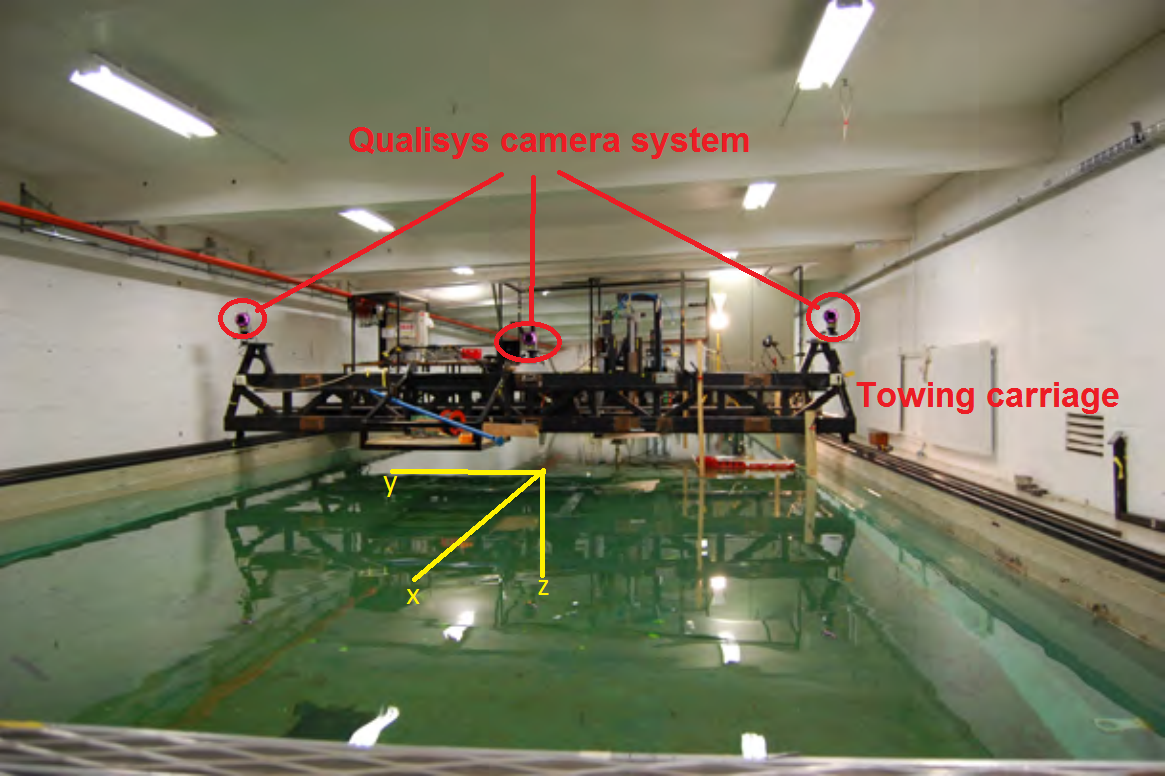
\includegraphics[width=0.95\textwidth]{mc_lab} \caption{\label{fig: Marine cybernetics laboratory basin}Marine cybernetics
laboratory basin}


\label{towing} 
\end{figure}


The laboratory is equipped for experimental testing of marine control
systems and hydrodynamic tests. It consists of a wave basin with an
advanced instrumentation package and a towing carriage. The basin,
depicted in Figure \ref{fig: Marine cybernetics laboratory basin},
has dimensions 40m x 6.45m x 1.5m (LxBxD).




\section{Equipment}


\subsection{Qualisys motion capture system}

Qualisys provides 6 degrees of freedom data tracking. The system has
millimeter precision, works in real time and is configured to 50Hz.

The positioning system consists of three Oqus high speed infrared
cameras registering infrared reflectors placed on the vessel. Peer-to-peer
(P2P) networking is used to transmit camera data to a dedicated computer
running Qualisys Track Manager (QTM) software. QTM performs triangulation
and broadcasts the vessel position over the HIL-lab network.


\subsection{Towing carriage}

The carriage runs at speeds up to 2m/s. It also has capability for
precise movement of models in 6 degrees of freedom and is thus suitable
for more specialized hydrodynamic tests.


\subsection{Wave generator}

\begin{table}
\centering{}%
\begin{tabular}{lll}
\hline 
 & Height {[}m{]} & Period T {[}s{]}\tabularnewline
\hline 
Regular waves & $H<0.25$ & 0.3 - 3.0\tabularnewline
Irregular waves & \textbf{$H_{s}<0.15$} & 0.6 - 1.5\tabularnewline
\hline 
\end{tabular}\caption{\label{tab:Wave generator capacity}Wave generator capacity}
\end{table}


The single paddle wave generator is controlled by a dedicated computer.
Available spectrum are first order Stoke, JONSWAP, Pierson-Moskowitz,
Bretschneider, ISSC and ITTC. Table \ref{tab:Wave generator capacity}
summarizes the generation capacity.

\clearpage{}


\section{Vessels}


\subsection{Cybership Enterprise 1}

\begin{figure}
\centering 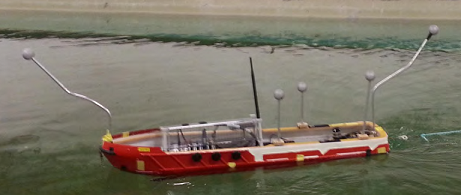
\includegraphics[width=0.95\textwidth]{CSE1_2.PNG} \caption{\label{fig: Cybership Enterprise 1}CS Enterprise 1}
\end{figure}


CSE1, depicted in Figure \ref{fig: Cybership Enterprise 1}, is a
model ship fitted with two Voith Schneider propellers (VSP) astern
and a bow thruster (BT). Its on-board control system consists of a
RPi and a cRIO, as in the HIL laboratory setup described in Chapter
\ref{sec: Marine HIL simulation laboratory}, in addition to three
electronic speed controllers (ESC) and four servos.


\subsubsection{High-level communication}

\begin{figure}
\centering 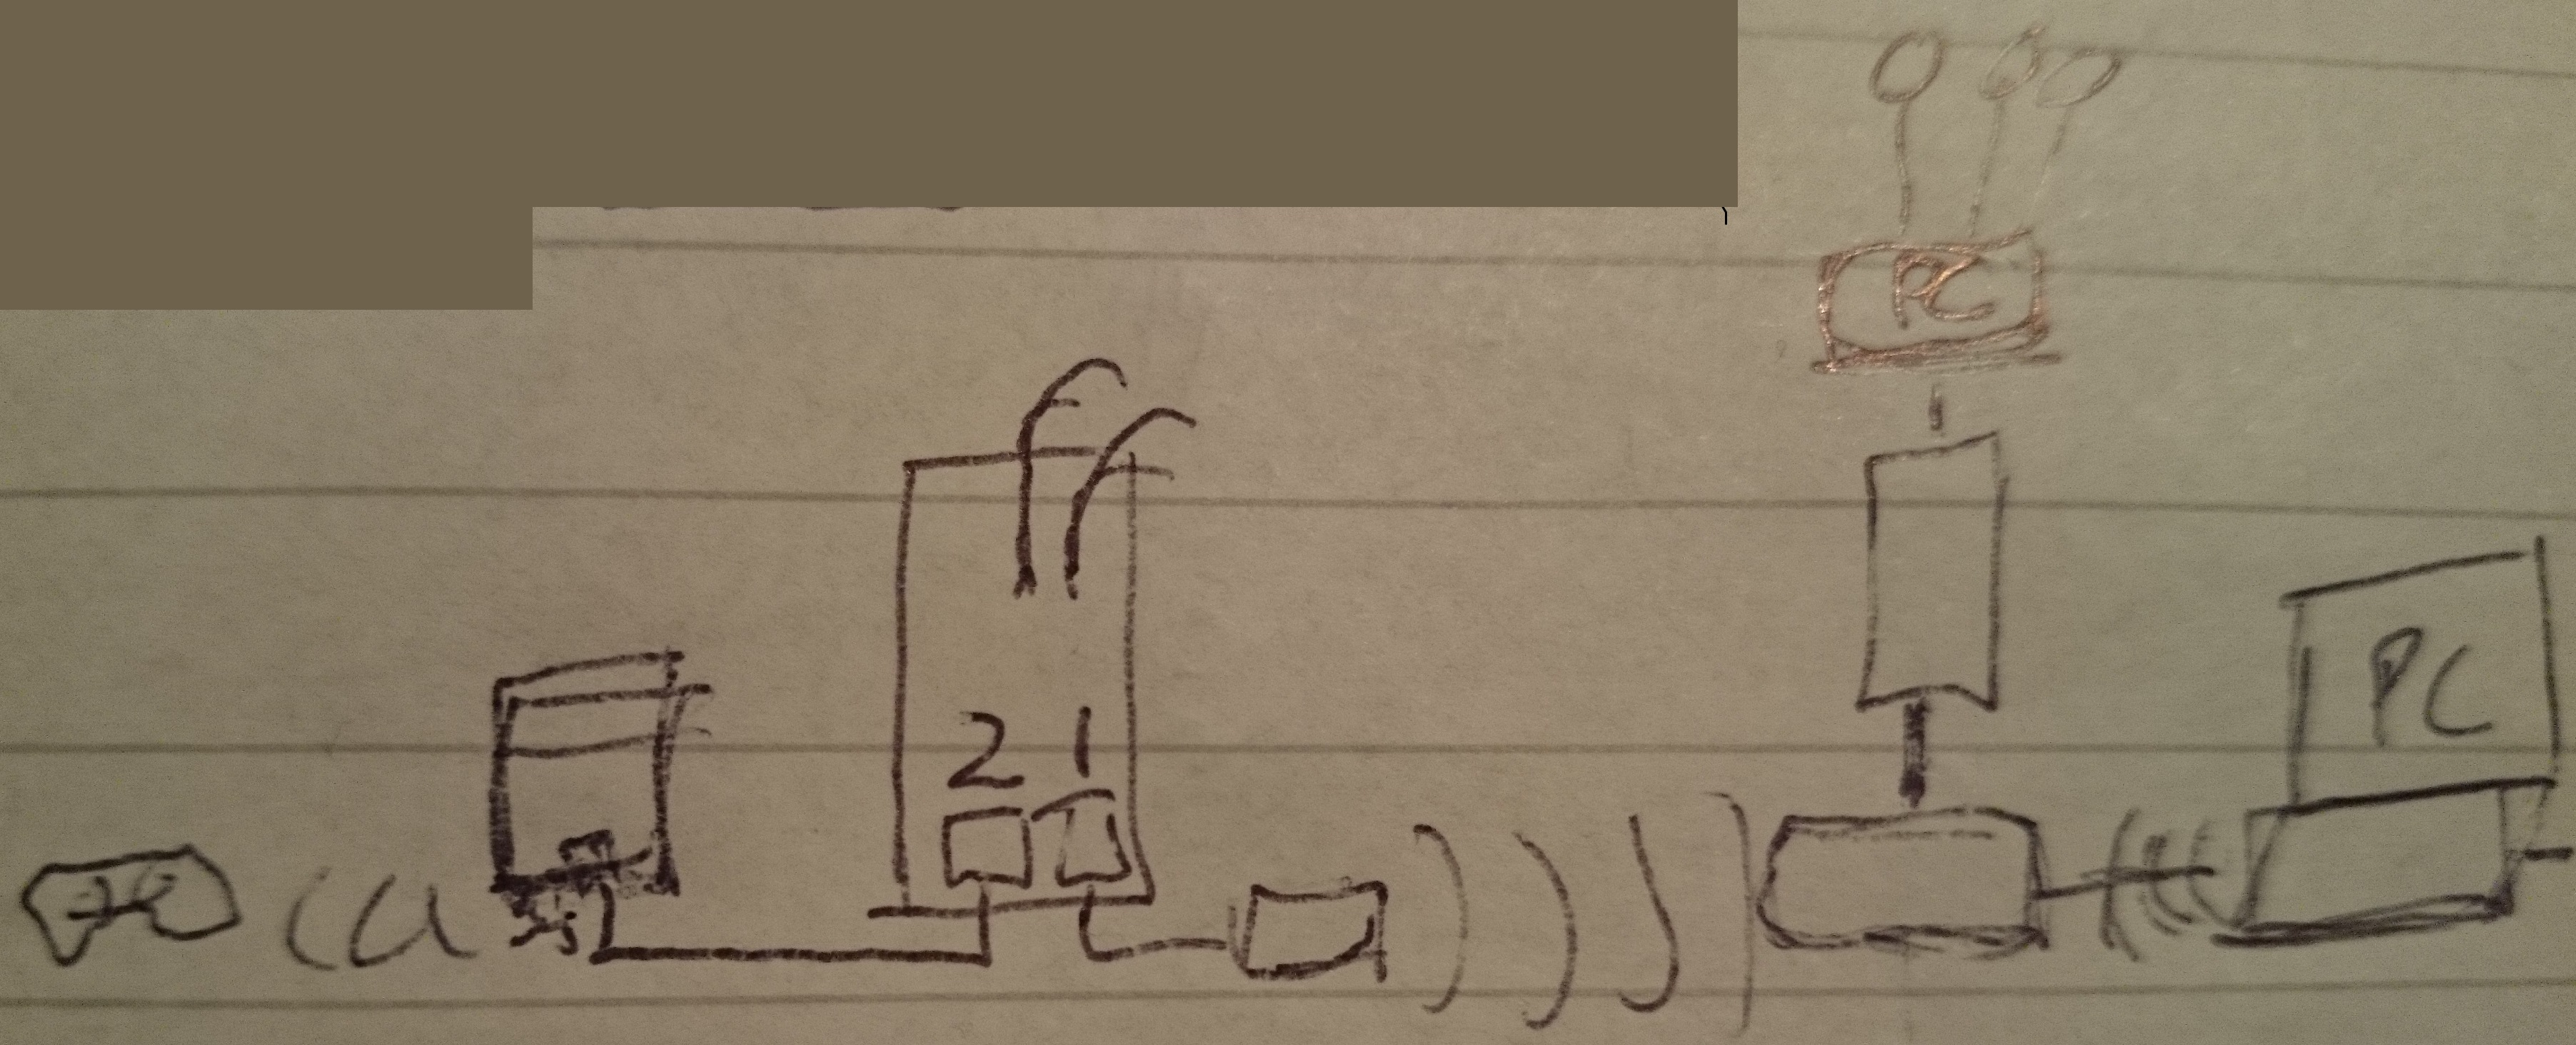
\includegraphics[width=0.95\textwidth]{setupCSE1} \caption{\label{fig: CSE1 communication} CSE1 communication}
\end{figure}


The communication is similar to the description of Section \ref{sub: HIL lab Communication},
with the exception of the wired Ethernet link between the cRIO and
the laptop. For CSE1 this link instead passes through a Wi-Fi bridge
to a wireless router to the laptop, as seen in Figure \ref{fig: CSE1 communication}.

Broadcast QTM positioning data is retrieved through the same wireless
network.


\subsubsection{Low-level communication}

The BT and VSP motor speeds are controlled by ESC. The ESC receive
their setpoints as a pulse-width modulated (PWM) signals from the
cRIO digital output module.

The VSP blade pitches are controlled by servos. The servos also receive
their setpoint as PWM signals.


\subsubsection{Control system}

\begin{figure}
\centering 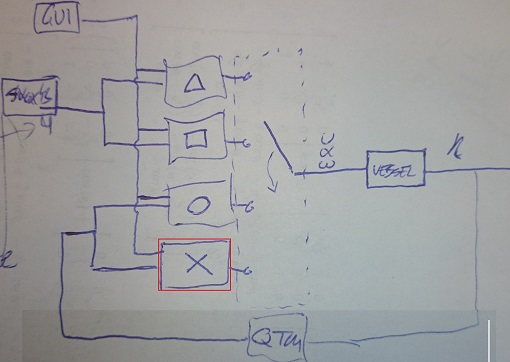
\includegraphics[width=0.8\textwidth]{CSE1_control_system}
\caption{\label{fig: CSE1 generic control system}CSE1 generic control system}
\end{figure}


\begin{table}
\centering{}%
\begin{tabular}{c>{\raggedright}p{6.5cm}}
\hline 
Sixaxis & Control mode\tabularnewline
\hline 

\includegraphics[scale=0.4]{sixaxis_triangle} & \textbf{Manual thruster control}

VSP speed: directional pad up/down $\pm0.1$

Left joystick: VSP1 thrust

Right joystick: VSP2 thrust

L2/R2: BT thrust\tabularnewline
\hline 

\includegraphics[scale=0.4]{sixaxis_square} & \textbf{Manual forces and moment control}

VSP speed: user interface button on/off

Left joystick: surge and sway forces

L2/R2: yaw moment\tabularnewline
\hline 

\includegraphics[scale=0.4]{sixaxis_circle} & \textbf{Basic dynamic positioning (DP)}

VSP speed: user interface button on/off

Setpoint: user interface

Gains: user interface\tabularnewline
\hline 

\includegraphics[scale=0.4]{sixaxis_cross} & \textbf{Student controller}

User implemented controller\tabularnewline
\hline 
\end{tabular}\caption{\label{tab: CSE1 control system modes}Generic control modes}
\end{table}


A diagram representation of CSE1's control system is given in Figure
\ref{fig: CSE1 generic control system}. The vessel can switch among
four control modes, summarized in Table \ref{tab: CSE1 control system modes}.
The first three controllers are predefined, while users may implement
their own controller in the fourth.

\begin{figure}
\centering 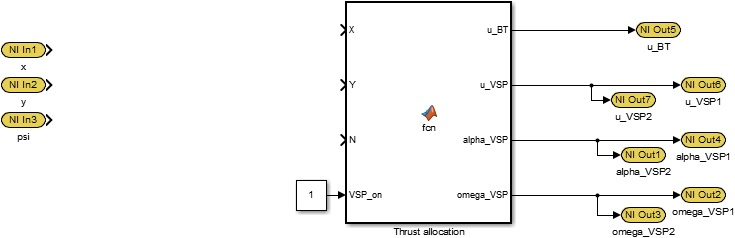
\includegraphics[scale=0.45]{CSE1_ctrl_student} \caption{\label{fig: CSE1 ctrl_student.slx}CSE1 \texttt{ctrl\_student.slx}
including thrust allocation}
\end{figure}


Implementation of the student controller is done in the \texttt{ctrl\_student.slx}
Simulink template, depicted in Figure \ref{fig: CSE1 ctrl_student.slx}.
Detailed implementation steps are given in Section \ref{sec: CSE1 Student controller implementation}.

The generic control system consists of several Simulink modules, the
details of which are given in Appendix \ref{sub: CSE1 Control software},
a FPGA driver, described in Appendix \ref{sub:Create-FPGA-target},
and two custom device drivers.

\clearpage{}


\subsection{Cybership 3}

-



\clearpage{}


\part{\label{part: Laboratory user guide}Laboratory user guide}


\chapter{HIL simulation and testing}


\section{Simulink model adaptation and compilation}

Complete the following steps to convert your model you created in
Simulink into a compiled model that runs on RT targets.

Version compatibility is an issue for VeriStand-Simulink interaction.
Mostly\footnote{It has been experience that MATLAB function blocks are not compatible
across versions. This results in build error message ``invalid object
ID''. The MATLAB function block code must then be copied and pasted
into a new MATLAB function block from the compatible version Simulink
Library Browser.} Simulink code may be programmed in any version of the MATLAB, compilation,
on the other hand, can only be done in version compatible with the
intended VeriStand version. See Section \ref{sub: Laptop software}.


\subsection{\label{sub: Simulink modeling}Modeling}


\subsubsection{Input and output}

In order for the model to interact with VeriStand, special input and
output blocks must be added to the block diagram\footnote{Ordinary input/source and output/sink blocks could be used at the
diagram top level. However, subsystem ports are only available when
using the VeriStand blocks.}. These are found in the Simulink Library Browser under NI VeriStand
Blocks.


\subsubsection{Initial conditions}

\begin{figure}[!h]
\centering 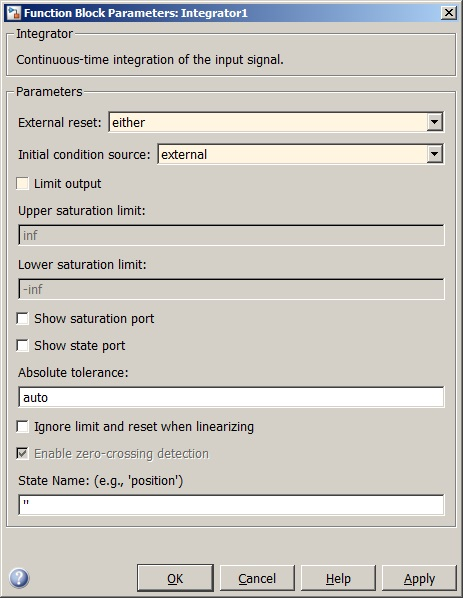
\includegraphics[scale=0.45]{simulink_integrator} \caption{Integrator function block parameters}


\label{fig: simulink integrator function block parameters} 
\end{figure}


If the simulation is to be run with different initial conditions,
one possible method is to allow external reset of the integrators.
This is done right-click the integrator and selecting Block Parameters
(Integrator) in the drop-down menu. Here, the reset condition is set.
The initial condition source should be external, as in Figure \ref{fig: simulink integrator function block parameters}.


\subsubsection{\label{sub:Real-time-data-logging}Real-time data logging}

\begin{figure}[!h]
\centering 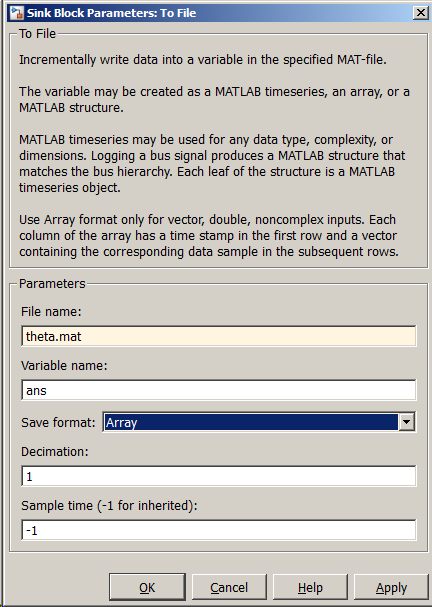
\includegraphics[scale=0.45]{simulink_tofile} \caption{To File block parameters}


\label{fig: simulink to file} 
\end{figure}


Model output can be saved to the cRIO, for later retrieval through
FTP, during simulation through a To File block. This block is found
in the Simulink Library Browser under Sinks. The output file name
is specified under the block parameters, as in Figure \ref{fig: simulink to file}.
The format should be set to Array, since the cRIO does not support
the Timeseries format.


\paragraph{Example:}

\begin{figure}[!h]
\centering 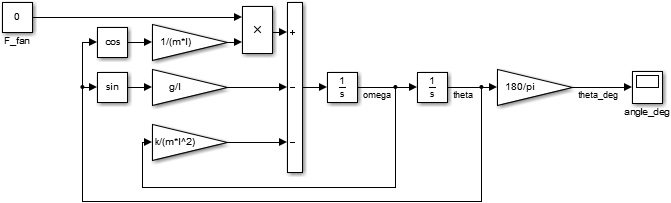
\includegraphics[scale=0.45]{simulink_before} \caption{Simulink model for offline simulation}


\label{fig: Simulink pendulum model} 
\end{figure}


\begin{figure}[!h]
\centering 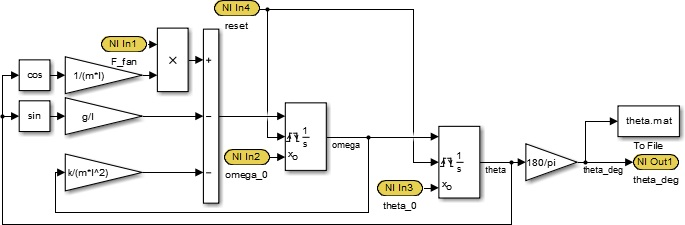
\includegraphics[scale=0.45]{simulink_after} \caption{Simulink model for adjusted for compilation}


\label{fig: simulink pendulum model for compilation} 
\end{figure}


For a simple pendulum, $\dot{\omega}=-\frac{g}{l}\sin\left(\theta\right)-\frac{k}{ml^{2}}\omega+\frac{F_{\text{fan}}}{ml}\cos\left(\theta\right)$,
the offline simulation block diagram could look as Figure \ref{fig: Simulink pendulum model}.
Figure \ref{fig: simulink pendulum model for compilation} shows the
same system adapted for VeriStand input, including reset and initial
conditions, and output. The VeriStand blocks are yellow. omega\_0
and theta\_0 are ports corresponding to the initial conditions $\left(\omega\left(0\right),\theta\left(0\right)\right)$.
The integrators take these values whenever reset is rising or falling.


\subsection{\label{sub: Simulink model configuration}Model configuration}

The code generation toolbox compiles the Simulink diagram to an output
shared library in {*}.out format\footnote{The {*}.out format is for targets running Wind River VxWorks real-time
operating system (RTOS) such as cRIO-9024, while dynamic link libraries
in {*}.dll format are for targets running IntervalZero Phar Lap ETS
RTOS such as cRIO-9081.}. Model configuration parameters must be adjusted before generating,
or building, the code.

\begin{figure}[!h]
\centering 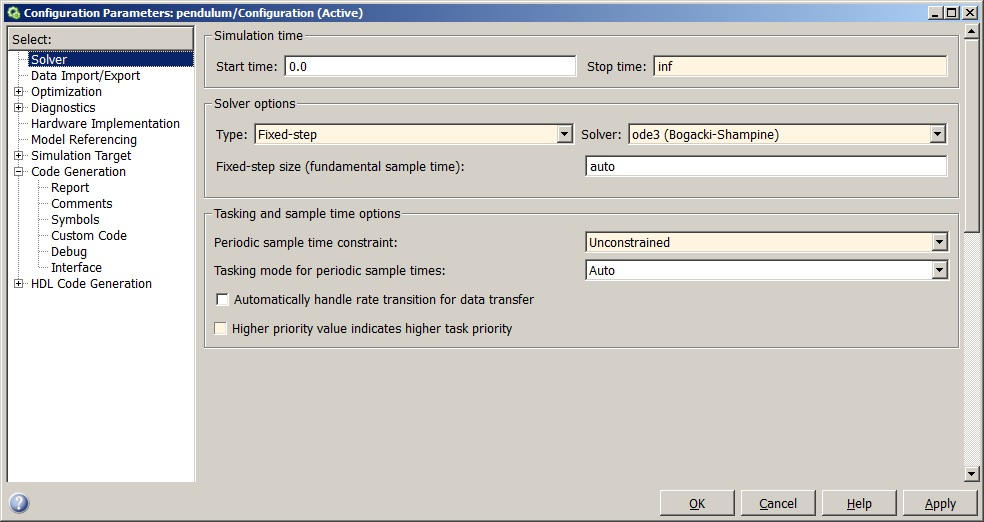
\includegraphics[scale=0.45]{simulink_settings_solver}
\caption{Simulink configuration parameters - solver}


\label{fig: simulink solver} 
\end{figure}


The solver stop time should be \texttt{inf} (infinity) if the model
is supposed to run until it is otherwise interrupted. The solver type
must be fixed step. If your model only performs arithmetical operations,
such as a mapping or transformation module would, the discrete solver
should be used. If the model contains continuous states, i.e. if you
have integrators, choose some differential equation solver such as
ode3 or ode4. See Figure \ref{fig: simulink solver}. Finally, the
step size can be set: for a target running at 100 Hz, such as the
cRIO-9024 default, a 0.01 step size results in the model running in
simulating 1 second pr. second\footnote{This can also be achieved by use of decimation, as described in Section
\ref{sub: Veristand System-setup}.}.

\begin{figure}[!h]
\centering 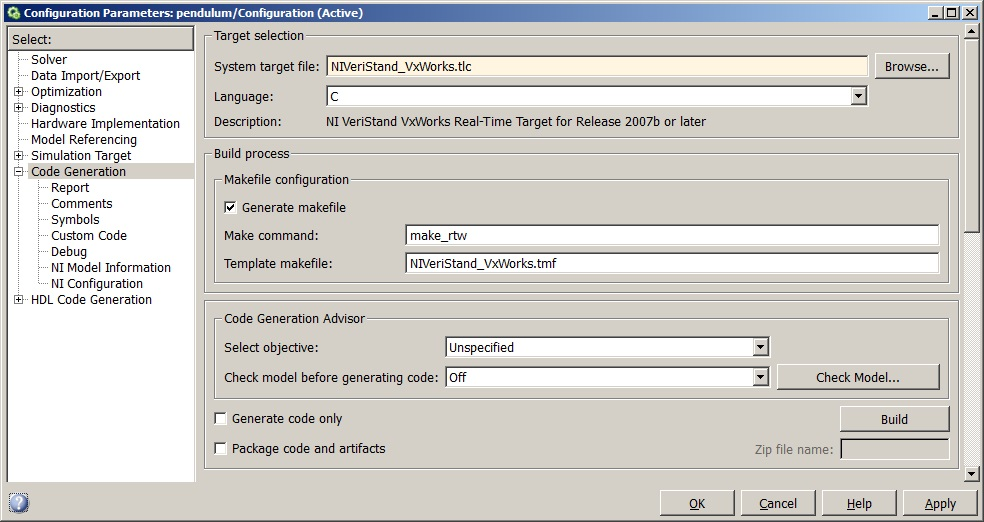
\includegraphics[scale=0.45]{simulink_settings_codegeneration}
\caption{Simulink configuration parameters - target selection}


\label{fig: simulink target selection} 
\end{figure}


The correct target file should be selected depending on the target
device. Select \texttt{NIVeriStand\_VxWorks.tlc} for VxWorks targets\footnote{For PharLap targets, select \texttt{NIVeriStand.tlc}.},
such as cRIO-9024, as in Figure \ref{fig: simulink target selection}.

\begin{figure}[!h]
\centering 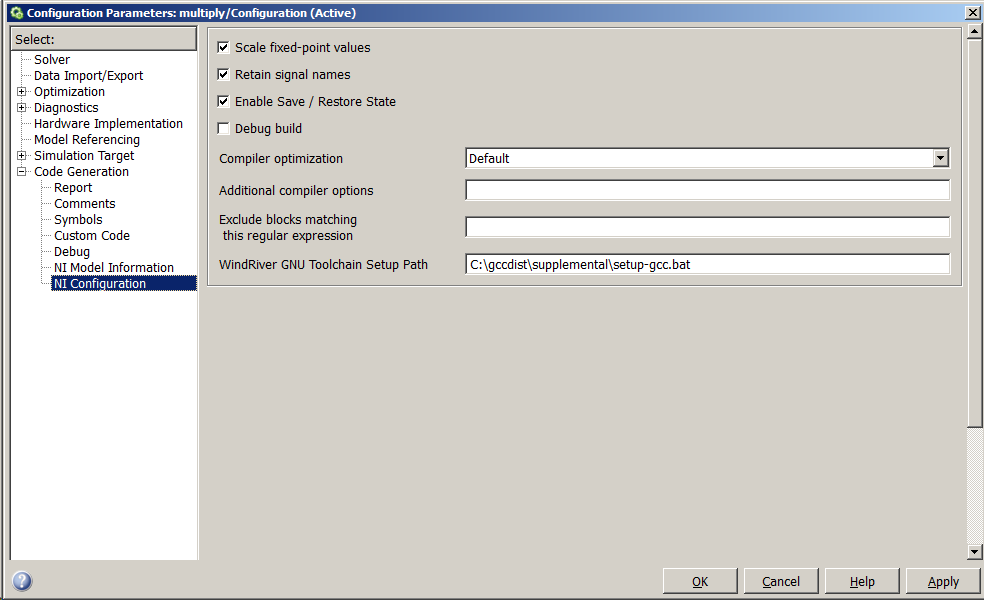
\includegraphics[scale=0.45]{simulink_settings_ni} \caption{Simulink model configuration - NI configuration}


\label{fig: simulink NI configuration} 
\end{figure}


The WindRiver GNU Toolchain must be present in the folder specified
under NI Configuration, as in Figure \ref{fig: simulink NI configuration}.


\subsection{\label{sub: Simulink model build}Build}

\begin{figure}[!h]
\centering 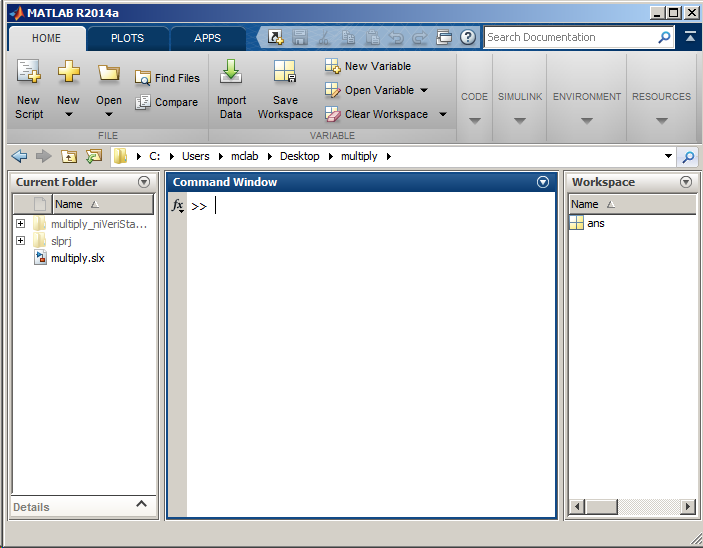
\includegraphics[scale=0.45]{matlab_command} \caption{MATLAB console}


\label{fig: matlab console} 
\end{figure}


The build output is placed in a subfolder in the MATLAB Current Folder.
The desired folder must therefore be active in the MATLAB main window,
as in Figure \ref{fig: matlab console}, before compiling. The build
subfolder name is {[}simulink model name{]}\_niVeriStand\_VxWorks\_rtw.

The build is done in in Simulink, either with the Build button in
the configuration window, by clicking the 
\includegraphics[scale=0.5]{simulink_build}
button, by the key combination \noun{Ctrl+B}, through the menu Code
\textgreater  C/C++ Code \textgreater  Build model, or by pushing
the icon button.

\clearpage{}


\section{Simulation configuration}

\begin{figure}
\centering 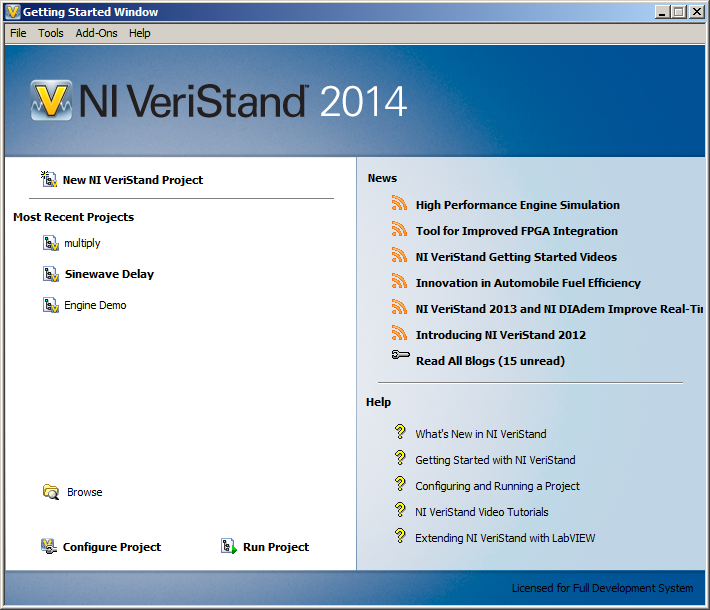
\includegraphics[scale=0.45]{veristand} \caption{VeriStand start screen}


\label{fig: veristand} 
\end{figure}


Simulations are set up, deployed and interfaced through VeriStand.
Figure \ref{fig: veristand} shows the start screen. Already configured
projects can be run directly from here, or reconfigured.


\subsection{Project creation}

To deploy model for the first time, click New NI VeriStand Project.
Give your new project a suitable name and location. 
\begin{figure}[h]
\centering 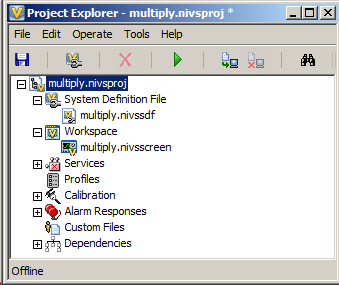
\includegraphics[scale=0.45]{veristand_projectexplorer}
\caption{VeriStand Project Explorer}


\label{fig: veristand project explorer} 
\end{figure}
 Clicking OK creates the project files in given location and opens
the Project Explorer, as in Figure \ref{fig: veristand project explorer}.
In this section, the example project name is multiply.


\subsection{\label{sub: Veristand System-setup}System setup}

To configure the setup which will run on the cRIO, open the System
Explorer by double-clicking the system definition file {[}project
name{]}.nivssdf.
\begin{enumerate}
\item 
\begin{figure}[h]
\centering 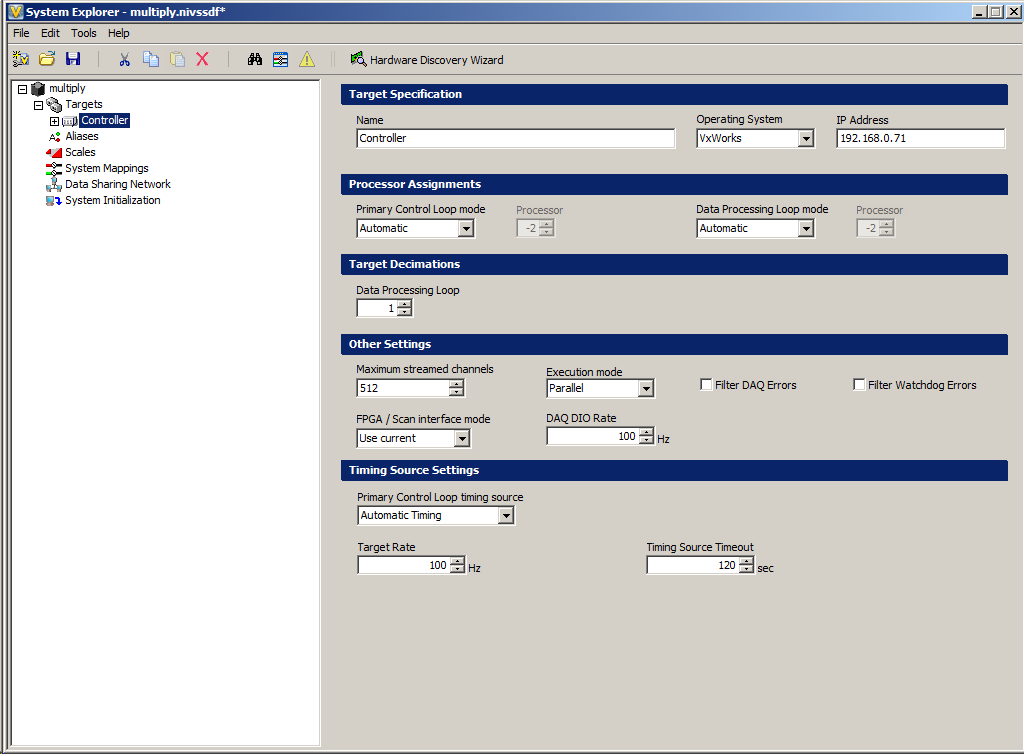
\includegraphics[scale=0.45]{veristand_systemexplorer_ip}
\caption{VeriStand - System Explorer - Controller}


\label{fig: veristand system explorer ip} 
\end{figure}
 Set the correct controller operating system and IP address, as in
Figure \ref{fig: veristand system explorer ip}. All HIL and MC lab
IP addresses are given in Table \ref{tab: IP addresses}. Also, note
the target rate.
\item 
\begin{figure}[h]
\centering 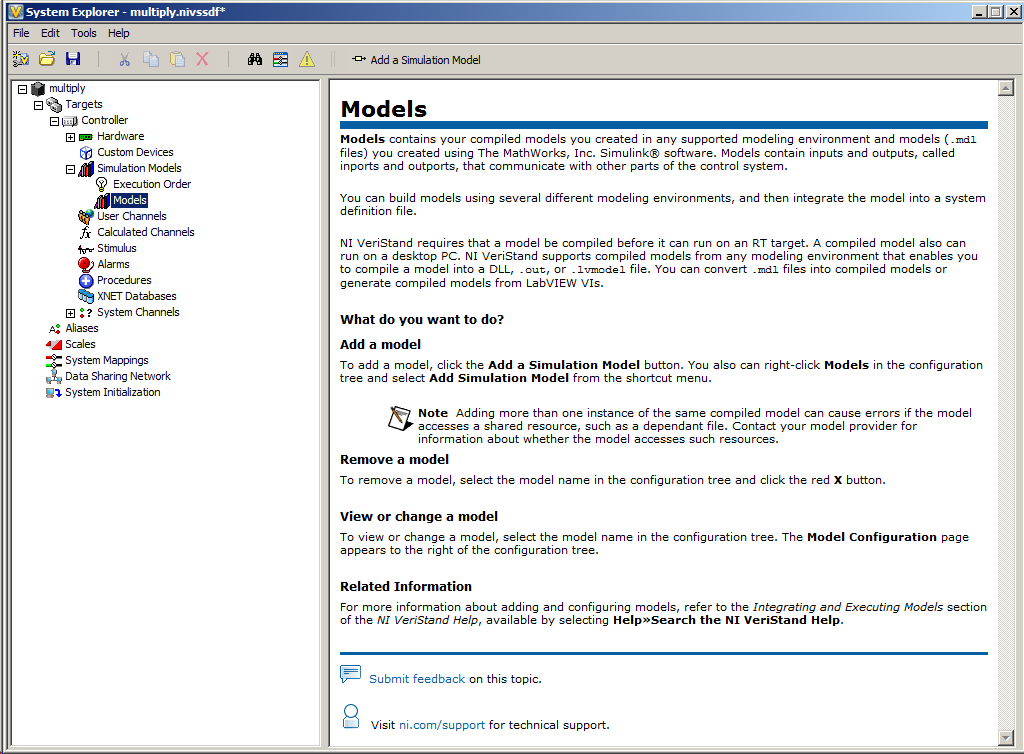
\includegraphics[scale=0.45]{veristand_systemexplorer}
\caption{VeriStand - System Explorer - Models}


\label{fig: veristand system explorer model} 
\end{figure}
 Click Add a Simulation Model, as seen at the top of Figure \ref{fig: veristand system explorer model}.
\begin{figure}[h]
\centering 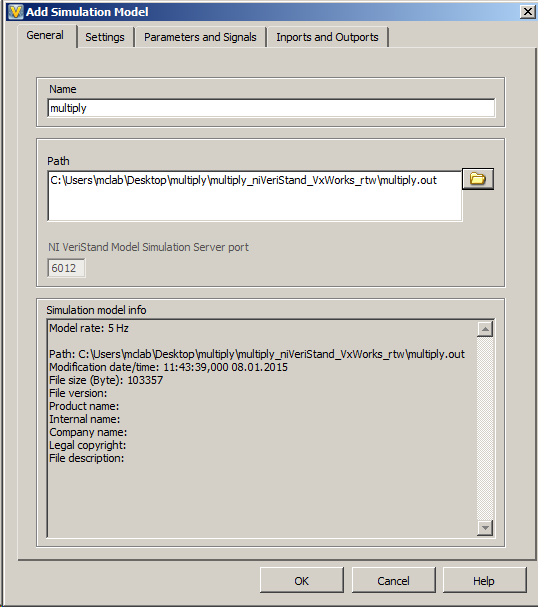
\includegraphics[scale=0.45]{veristand_systemexplorer_model}
\caption{VeriStand - System Explorer Model}


\label{fig: veristand system explorer model 2} 
\end{figure}
 Browse to the output of the Simulink compilation, as seen in Figure
\ref{fig: veristand system explorer model 2}. Finally, click Auto
Select Decimation to make sure the model runs at the intended rate.\\
Repeat if several models should run simultaneously.
\item Add custom devices, such as network input, by right clicking the custom
device pane and choosing the required device\footnote{If the required device is not present, refer to the device driver
installation instructions in Section \ref{sub: Installing custom device driver}.}. 
\begin{figure}[!h]
\centering \includegraphics[scale=0.45]{\string"veristand custom driver select\string".png}
\caption{Custom device selection}


\label{fig: veristand system explorer custom device selection-1} 
\end{figure}
 Figure \ref{fig: veristand system explorer custom device selection-1}
shows an example with the Sixaxis (WL\_Joystick) device. Upon selection,
a subfolder with the device name appears in the tree with signals
listed inside it.
\item Configure mappings, by pushing the 
\includegraphics[scale=0.8]{veristand_sysex_mappingbtn}
icon at the top of the window, to connect signals between custom devices,
FPGA and models.
\begin{figure}[!h]
\centering \includegraphics[scale=0.45]{\string"veristand mapping2\string".png}
\caption{VeriStand System Configuration Mappings}


\label{fig: veristand mappings-1} 
\end{figure}
 Expand the trees to find the desired signals and click Connect, as
in Figure \ref{fig: veristand mappings-1}.
\item Save and close to return to the Project Explorer.
\end{enumerate}

\subsection{\label{sub: Create computer interface}Create computer interface}

To configure the computer interface, open the Workspace editor by
double-clicking the workspace file {[}project name{]}.nivsscreen.
The blank workspace pops up.
\begin{enumerate}
\item Enter Edit mode by \noun{Ctrl+M} or Screen \textgreater  Edit Mode.
\item Click the Workspace Control pane on the left side to access indicators,
controls and such.
\item Drag and drop the desired item to the desired position in the workspace.
Select the corresponding signal in the pop-up dialog.
\item Close the Workspace editor.
\end{enumerate}
\clearpage{}


\section{Deployment and simulation}


\subsection{Run}

Deploy by tapping the F6 key, or 
\includegraphics[scale=0.8]{veristand_deploy}
button, or Operate \textgreater  Deploy. A dialog box appears. Upon
successful deployment, the workspace pops up.


\subsection{User interface side data logging}

For reliability, it is recommended to log data directly on the cRIO
during simulation, as described in Section \ref{sub:Real-time-data-logging}.
It is also possible to log via the laptop user interface.

\begin{figure}[h]
\centering 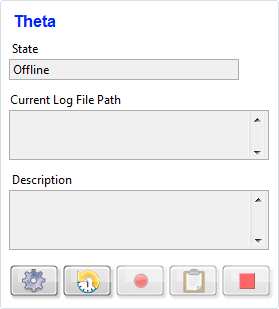
\includegraphics[scale=0.45]{veristand_ws_logging} \caption{Logging Control}


\label{fig: veristand workspace logging control} 
\end{figure}


A Logging Control, as seen in Figure \ref{fig: veristand workspace logging control},
must be added to the workspace to export data from the simulation.
The control is added as described in Section \ref{sub: Create computer interface}.

\begin{figure}[h]
\centering 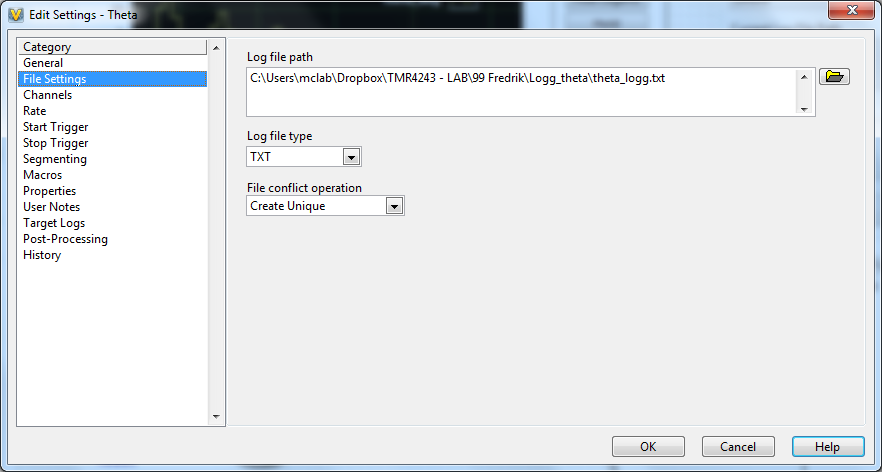
\includegraphics[scale=0.45]{veristand_ws_logging_file}
\caption{Logging Control file settings}


\label{fig: veristand workspace logging file} 
\end{figure}
\begin{figure}[h]
\centering 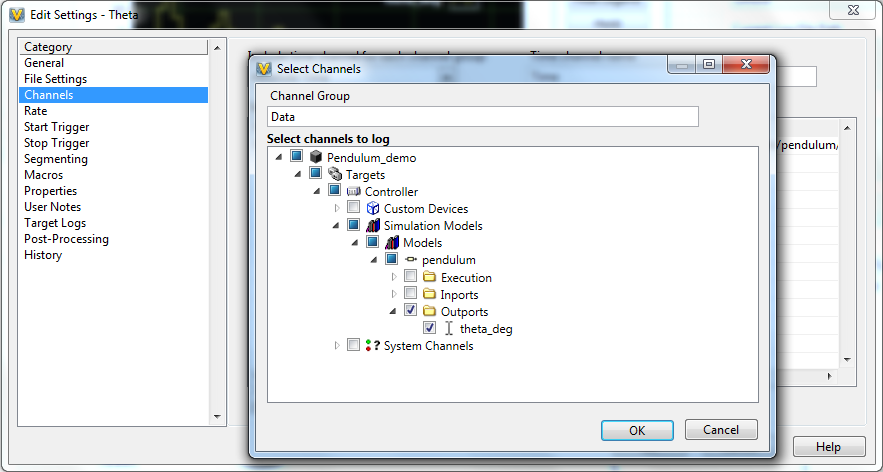
\includegraphics[scale=0.45]{veristand_ws_logging_add_ch}
\caption{Logging Control add channel}


\label{fig: veristand workspace logging channels} 
\end{figure}


Once the control is added, a pop-up window allows to edit the settings.
The log file path is specified under File Settings, see Figure \ref{fig: veristand workspace logging file}.
Under Channels, the desired channels can be selected and added, as
in Figure \ref{fig: veristand workspace logging channels}.


\subsection{Stop}


\includegraphics[scale=0.8]{veristand_undeploy} button


\subsection{FTP data retrieval}

Data logged on the cRIO through To File blocks can be retrieved after
simulation over FTP with software such as WinSCP.

\begin{figure}[h]
\centering 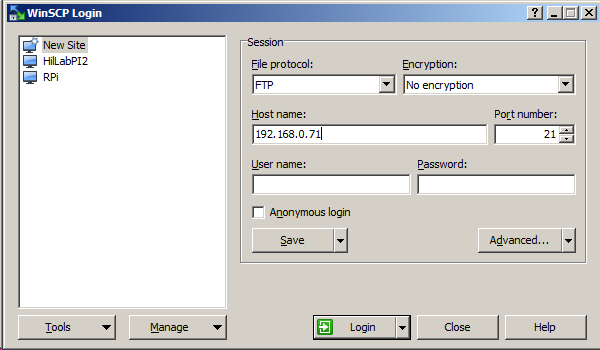
\includegraphics[scale=0.45]{WinSCP_login} \caption{\label{fig: WinSCP login}WinSCP login}
\end{figure}


To connect to the cRIO, the correct IP must be specified, as in Figure
\ref{fig: WinSCP login}. For the standard HIL setup, the user name
and password are blank.

\begin{figure}[h]
\centering 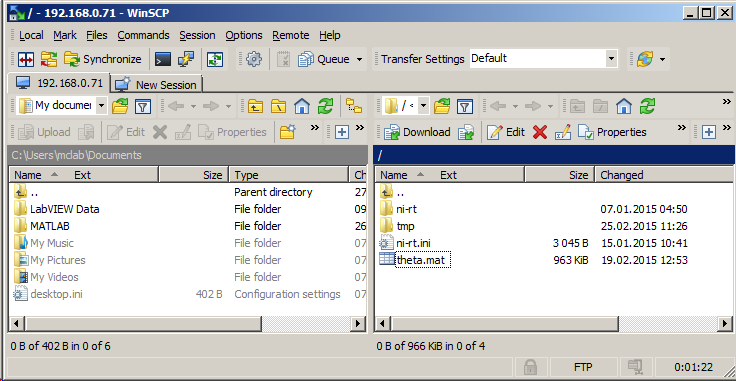
\includegraphics[scale=0.45]{WinSCP} \caption{\label{fig: WinSCP}WinSCP}
\end{figure}


Logged data with file names corresponding to the To File block names
are located on the cRIO root, as seen in the right pane of Figure
\ref{fig: WinSCP}. Data is transferred to the laptop by drag and
drop to the desired location in the left pane.



\clearpage{}


\chapter{CSE1 model scale testing}


\section{Safety - hazards and measures}


\subsection{Personnel injury}


\subsubsection{Drowning}

It is required to have two or more persons present when using the
basin.


\subsubsection{Electric shock}

The towing catenary should not be approached or touched.


\subsubsection{Carriage collision}

It is forbidden to run the towing carriage when there are people alongside
the basin.


\subsubsection{Thruster blade cuts}

CSE1 must stay in the water as long as actuators are active. Before
removing the vessel from the water, the control system must be stopped
and the VeriStand project undeployed.


\subsection{Material damage}


\subsubsection{Cybership Enterprise 1}


\paragraph{Water damage}

CSE1 is not waterproof and has excessive thrust capability which can
inflict large roll angles. The risk of water on deck is reduced through
thrust limitation and HIL testing before application of new control
algorithms. 


\paragraph{Propeller dry running}

BT must only be run in water. Before removing the vessel from the
water, the control system must be stopped and the VeriStand project
undeployed.


\paragraph{Loss of laptop control }

Wireless network instability may result in loss of connection between
the laptop user interface and the cRIO. In this event, fall back to
manual thruster control, by pushing 
\includegraphics[scale=0.4]{sixaxis_triangle}
on the Sixaxis.


\paragraph{Loss of position measurement}

-


\paragraph{Total loss of control}

Pull the vessel with a boat hook. Keep the CSE1 in water while disconnecting
batteries.


\subsubsection{Towing carriage}

Stop before automatic stop at high speeds.

\clearpage{}


\section{\label{sec: CSE1 Student controller implementation}Student controller
implementation}
\begin{enumerate}
\item Unzip the CSE1 Veristand Project {\texttt{CSE1.zip}} to \texttt{C:\textbackslash{}CSE1\textbackslash{}}.\footnote{Other paths are possible but require changing all VeriStand project
paths.}
\item Simulink implementation and compilation

\begin{enumerate}
\item Update {\texttt{ctrl\_student.slx}} according to your controller
design. Additional input and output, resets and data logging may be
added, as described in Section \ref{sub: Simulink modeling}.\\
Do not alter the predefined input and output: x, y, psi, u\_BT, u\_VSP1,
u\_VSP2, alpha\_VSP1, alpha\_VSP2, omega\_VSP1 and omega\_VSP2.
\item Select a suitable solver, as described in Section \ref{sub: Simulink model configuration}.\\
The remaining configuration, such as target selection is preselected
in the file.
\item Compile the model as described in Section \ref{sub: Simulink model build}.
The MATLAB current folder should be \texttt{C:\textbackslash{}CSE1\textbackslash{}},
in order to ensure that the resulting \texttt{.out} file is created
in \texttt{C:\textbackslash{}CSE1\textbackslash{}ctrl\_student\_niVeriStand\_VxWorks\_rtw}.
\end{enumerate}
\item CSE1 Veristand Project configuration

\begin{enumerate}
\item Open {\texttt{CSE1.nivsproj}}\footnote{Not \texttt{CSE1.nivssdf}, since not only the system definition should
be altered.} to access the project.
\item Update {\texttt{ctrl\_student.out}}:

\begin{enumerate}
\item Open the System Explorer by double-clicking the system definition
file \texttt{CSE1.nivssdf}.
\item 
\begin{figure}
\centering 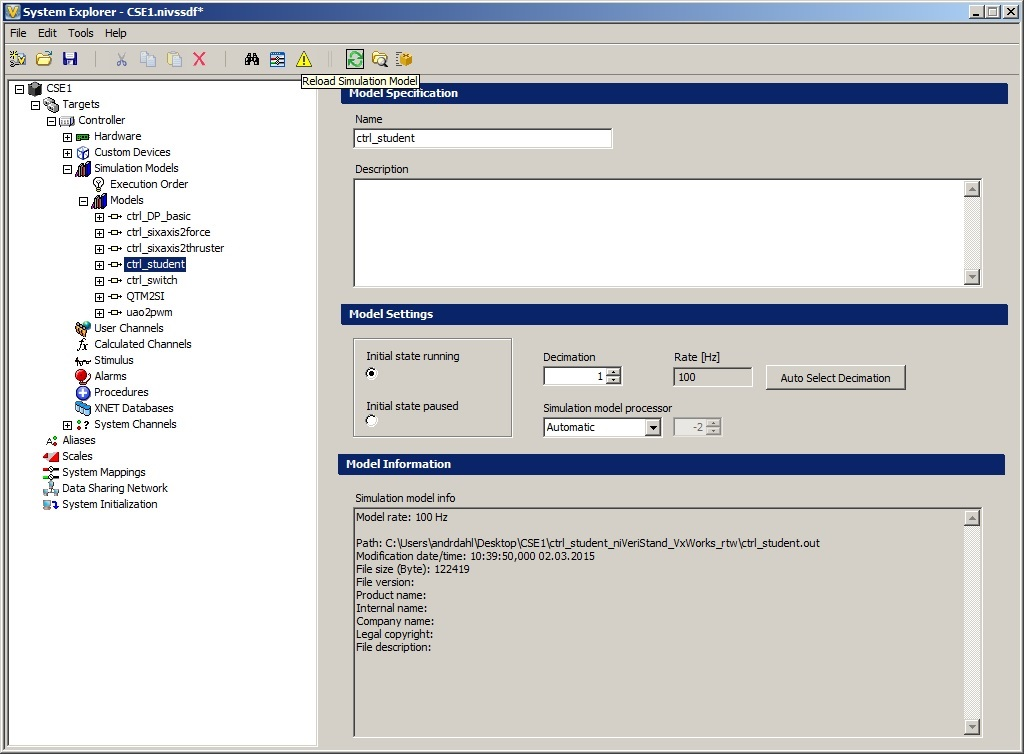
\includegraphics[scale=0.45]{CSE1_update_ctrl_studtent}
\caption{\label{fig: CSE1 simulation models}CSE1 Veristand Project simulation
models}
\end{figure}
Browse the left pane tree, as seen in Figure \ref{fig: CSE1 simulation models},
and select ctrl\_student. Refresh by pushing the 
\includegraphics[scale=0.8]{veristand_refresh}
icon.
\item If necessary, add mappings.\\
Do not change the existing mappings. Position input (x, y, psi) and
controller output (u\_BT, u\_VSP1, u\_VSP2, alpha\_VSP1, alpha\_VSP2,
omega\_VSP1, omega\_VSP2) are already mapped as necessary.
\item Save and close to return to the Project Explorer.
\end{enumerate}
\item 
\begin{figure}
\centering 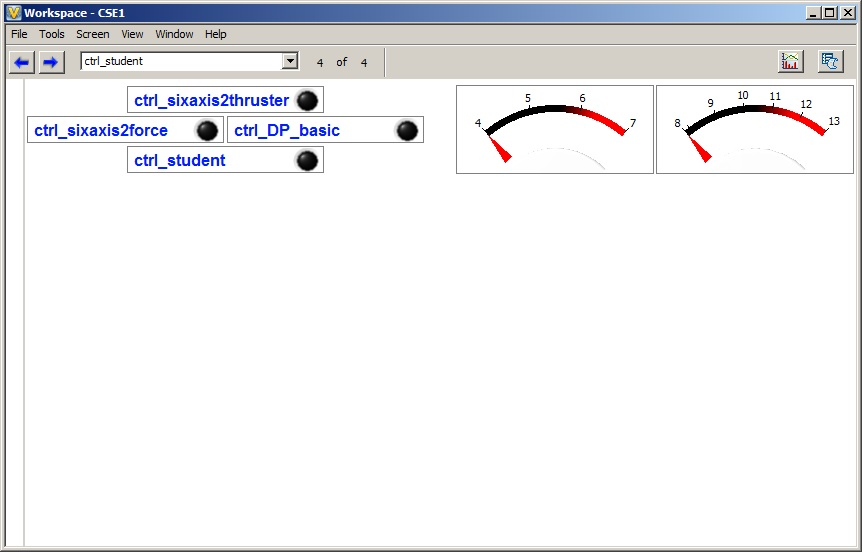
\includegraphics[scale=0.45]{CSE1_student_workspace}
\caption{\label{fig: CSE1 student_ctrl workspace}CSE1 Veristand Project ctrl\_student
workspace}
\end{figure}
Implement a suitable workspace, as described in Section \ref{sub: Create computer interface},
for your controller in control screen 4: ctrl\_student. Figure \ref{fig: CSE1 student_ctrl workspace}
shows control screen 4 before customization.
\end{enumerate}
\end{enumerate}
\clearpage{}


\section{Ship launching procedure - before sailing}


\subsection{Power up and connection}
\begin{enumerate}
\item \noindent Place the batteries adjacent to the watertight box: main
battery battery (12 V) astern and secondary battery (6 V) in the bow.
\item \noindent Connect main battery: first the red wire to the red/positive
pole, then the black wire to the black/negative pole\footnote{The connection order of the wires should not matter. However, experiences
favor the this order of connection.}.\\
cRIO LED nr.1 (power) will light up green.
\item Wait for cRIO and RPi start up.\\
When complete, the Bluetooth dongle blue LED blinks evenly at approximately
1 Hz.
\item Turn on Sixaxis by pushing the PS3 button.\\
When succesfully connected, the Bluetooth dongle blue LED is almost
constantly lit and the Sixaxis' red LEDs 1, 2, 3, and 4 blink at approximately
2 Hz.
\item Connect the seconday battery: red wire to the red/positive pole, then
the black wire to the black/negative pole.\\
The Wifi bridge Power LED will light up green.
\item Wait for WiFi connection to HILlab network.\\
When connected, the Wifi bridge WLAN green LED turns on.
\item 
\begin{figure}[h]
\centering 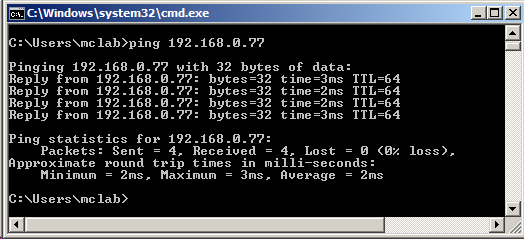
\includegraphics[scale=0.45]{cRIO_ping} \caption{\label{fig: ping}Ping, successful access to CSE1}
\end{figure}
Verify laptop access: ping the CSE1 IP in the command promt, as in
Figure \ref{fig: ping}. While the round trip times may vary, it is
essential to have 0\% loss.
\item Gently place the vessel in the basin, avoiding any water splashes.
\end{enumerate}



\subsection{Positioning system}

\clearpage{}


\section{Deploy control system}

\todo{Veristand osv}

\clearpage{}


\section{Ship docking procedure - after sailing}

Undeploy the running project to disable all actuators.

Lift out of water avoiding water on rail.

Put CSE1 in its stand. The vessel should not be left on the water
for extensive periods, i.e. overnight.

Remove and put used batteries to charge. Load fresh batteries in vessel.

Connect the Sixaxis gamepad to the laptop for charging.



\FloatBarrier

\newpage{}


\part{\label{part: Lab exercises}TMR4243 exercises and expected results}

General report requirements.


\chapter{Pendulum lab}

Adjust Simulink model for VeriStand.

Deploy

Create suitable workspace

Actuate fan manually.

Simulate to get same results as Simulink.

Export data

Try with handed out model (surprises).

\FloatBarrier

\newpage{}


\chapter{Internal dynamics lab}

\FloatBarrier

\newpage{}


\chapter{Estimation lab}


\section{Objective}

Teste konseptet, tau inputt,


\section{Theory and simulation}

Pure sway and surge dampings

\begin{equation}
d_{\text{pure surge}}=d_{11}u\label{eq: pure surge damping}
\end{equation}


\begin{equation}
d_{\text{pure sway}}=d_{22}v\label{eq: pure sway damping}
\end{equation}
Common DP model
\begin{equation}
d_{11}\left(u\right)=-X_{u}-X_{\left\vert u\right\vert u}\left\vert u\right\vert -X_{uuu}u^{2}\label{eq: Fossen d_11}
\end{equation}
\begin{equation}
d_{22}\left(v,r\right)=-Y_{v}-Y_{\left\vert v\right\vert v}\left\vert v\right\vert -Y_{vvv}v^{2}-Y_{\left\vert r\right\vert v}\left\vert r\right\vert \label{eq: Fossen d_22}
\end{equation}
however, Fitting the drag force to experiemtal results yields the
best fit for
\begin{equation}
d_{11}\left(u\right)=-X_{u}-X_{uu}u-X_{uuu}u^{2}\label{eq: CSE1 HIL d_11}
\end{equation}
\begin{equation}
d_{22}\left(v\right)=-Y_{v}-Y_{vv}v-Y_{vvv}v^{2}\label{eq: CSE1 HIL d_22}
\end{equation}
with parameters as listed in Table \ref{tab: CSE1-hydrodynamic}.

\begin{table}
\begin{centering}
\begin{tabular}{crcr}
\multicolumn{2}{c}{Surge} & \multicolumn{2}{c}{Sway}\tabularnewline
\midrule 
$X_{u}$  & $-0.6555$  & $Y_{v}$  & $-1.330$ \tabularnewline
$X_{uu}$  & $0.3545$  & $Y_{vv}$  & $-2.776$ \tabularnewline
$X_{uuu}$  & $-3.7870$  & $Y_{vvv}$  & $-64.910$ \tabularnewline
\bottomrule
\end{tabular}
\par\end{centering}

\caption{\label{tab: CSE1-hydrodynamic}CSE1 hydrodynamic damping parameters}
\end{table}



\subsection{Tasks}
\begin{enumerate}
\item Use \eqref{eq: CSE1 HIL d_11} to find the thurst required to achieve
$0.6\text{ m/s}$ and $-0.6\text{ m/s}$ in surge velocity. Equivalently
with \eqref{eq: CSE1 HIL d_22} and velocities $0.3\text{ m/s}$ and
$-0.3\text{ m/s}$ in sway.


\[
X=-X_{u}u-X_{uu}u^{2}-X_{uuu}u^{3}
\]
\[
Y=-Y_{v}v-Y_{vv}v^{2}-Y_{vvv}v^{3}
\]


\item Motion control


switche mellom sway og surge fixed, alltid rotasjon fixed

\item Surge hydrodynamics$\left[\begin{array}{c}
X_{\dot{u}}\\
X_{u}\\
X_{\left|u\right|u}
\end{array}\right]$


design reasonable towing input

\item Sway hydrodynamics$\left[\begin{array}{c}
Y_{\dot{v}}\\
Y_{v}\\
Y_{\left|v\right|v}
\end{array}\right]$
\item Real surge towing data$\left[\begin{array}{c}
X_{u}\\
X_{\left|u\right|u}
\end{array}\right]$
\end{enumerate}

\subsection{Specific report requirements}


\section{Hardware-in-the-loop simulation}


\subsection{Tasks}
\begin{enumerate}
\item Motion control


discrete and switcing controller

\item Real-time application configuration 

\begin{enumerate}
\item Create a VeriStand simulation project including the compiled control
system ctrl\_student.out and the CSE1 HIL model. i. Map control signals
and measurements according to Tables 1 and 2, respectively.
\item Develop a suitable graphical user interface.
\end{enumerate}
\item Simulate to estimate surge, sway and yaw hydrodynamic parameters separately
with the discrete controller as control input. Suitable velocity thresholds
are u = 0; 25, v = 0; 20 and r = 0; 30. Keep CSE1 within the line
f(x; y) j1 x 7:5; y = 0:25g to ensure position measurements.
\end{enumerate}

\subsection{Specific report requirements}


\section{Model scale testing}

HIL

\FloatBarrier

\newpage{}


\chapter{The maneuvering lab}



\FloatBarrier

\newpage{}

\appendix

\part{\label{part: Equipment setup and configuration}Equipment setup and
configuration}


\chapter{HIL lab setup}


\section{\label{sub: cRIO setup}cRIO}

The cRIO runs Wind River VxWorks real-time operating system.


\subsection{Ethernet ports}

The cRIO has two Ethernet ports the primary communicates with the
PC and the secondary with the Raspberry PI.


\subsubsection{Primary}

Set fixed IP, set fixed IP on HIL-computers


\subsubsection{Enabling the secondary ethernet port}


\begin{enumerate}
\item Start \emph{NI MAX}
\item In the left pane tree, select the cRIO under \emph{Remote Systems}
\item Open the \emph{Network Settings} tab (located at the bottom of the
window)
\item Set \emph{Adapter Mode} to \emph{TCP/IP Network}
\item Set \emph{Configure IPv4 Address} to \emph{Static}
\end{enumerate}
\begin{figure}[!h]
\centering \includegraphics[scale=0.45]{\string"Screenshots/Screenshot 2015-01-16 14.10.14\string".png}
\caption{NI MAX - Network Settings}


\label{fig: network settings} 
\end{figure}


\FloatBarrier

\newpage{}


\subsection{Update cRIO software}

To be able to run the models on the cRIO, the software version on
the cRIO and PC must match. In addition you must install the NI Veristand
Engine. Software changes on the cRIO is handled in NI Max.


\subsubsection{Update}
\begin{enumerate}
\item Open NI Max
\item Find your cRIO on the left hand side and click it
\item Click Software, and then Add/Rem ove Software located on the top pane,
see Figure \ref{fig: Software update 1}
\item A new window will now open. Choose the option that matches your LabVIEW/Veristand
edition (in our case 14.0 or 14.0.1) under LabVIEW Real-Time 14.0.0
and click next. See Figure \ref{fig: NI MAX - Software Update 2}
\item Click next without making any changes\ref{fig: NI MAX - Software Update 1-3}
\item Click next without making any changes\ref{fig: NI MAX - Software Update 4}
\item Wait for the installtion to finish and the cRIO to reboot
\end{enumerate}
\begin{figure}[!h]
\centering \includegraphics[scale=0.45]{\string"Screenshots/Screenshot 2015-01-16 14.12.35\string".png}
\caption{NI MAX - Software Update 1}


\label{fig: Software update 1} 
\end{figure}


\begin{figure}[!h]
\centering \includegraphics[scale=0.45]{\string"Screenshots/Screenshot 2015-01-16 14.12.51\string".png}
\caption{NI MAX - Software Update 1}


\label{fig: NI MAX - Software Update 2} 
\end{figure}


\begin{figure}[!h]
\centering \includegraphics[scale=0.45]{\string"Screenshots/Screenshot 2015-01-16 14.13.03\string".png}
\caption{NI MAX - Software Update 3}


\label{fig: NI MAX - Software Update 1-3} 
\end{figure}


\begin{figure}[!h]
\centering \includegraphics[scale=0.45]{\string"Screenshots/Screenshot 2015-01-16 14.15.22\string".png}
\caption{NI MAX - Software Update 4}


\label{fig: NI MAX - Software Update 4} 
\end{figure}


\FloatBarrier


\subsubsection{NI Veristand Engine}
\begin{enumerate}
\item Repeat step 1-3 from the previous guide
\item Now you choose Custom Software installation in the menu, see Figure
\ref{fig: NI Veristand Engine installation 1}
\item Ignore the warning, See Figure \ref{fig: NI Veristand Engine installation 1-1}
\item Locate NI Veristand Engine 2014 0.0 and click install feature. See
Figure \ref{fig: NI Veristand Engine installation 1-2}
\item Click your way through the rest of the installation and let the cRIO
reboot.
\end{enumerate}
\begin{figure}[!h]
\centering \includegraphics[scale=0.45]{\string"Screenshots/Screenshot 2015-01-16 14.20.27\string".png}
\caption{NI MAX - NI Veristand Engine installation 1}


\label{fig: NI Veristand Engine installation 1} 
\end{figure}


\begin{figure}[!h]
\centering \includegraphics[scale=0.45]{\string"Screenshots/Screenshot 2015-01-16 14.20.39\string".png}
\caption{NI MAX - NI Veristand Engine installation 1}


\label{fig: NI Veristand Engine installation 1-1} 
\end{figure}
\begin{figure}[!h]
\centering \includegraphics[scale=0.45]{\string"Screenshots/Screenshot 2015-01-16 14.21.07\string".png}
\caption{NI MAX - NI Veristand Engine installation 1}


\label{fig: NI Veristand Engine installation 1-2} 
\end{figure}


\clearpage{}


\subsection{\label{sub:Create-FPGA-target}Create FPGA target and XML}

If you do not haav a Veristand FPGA target at your disposal, follow
the steps below. If you have a target available and just need to install
it in NI Veristand, please jump to the next subsection
\begin{enumerate}
\item Open LabVIEW and create new project. We have done this in LabVIEW
2013 because of some instalation issues with LabVIEW 2014, but the
procedure should be the same for both editions.
\item Choose NI Veristand FPGA Project in project templates and proceed.
\item Choose CompactRIO Reconfiguarble Embedded System and click next.
\item You will now get the choice between letting LabVIEW detect your cRIO
system or configure it yourself. If you are connected to the cRIO
and it has all of the I/O ports connected, the option ``Discover
existing system'' is simpler and therefore recommneded. If you do
not have your cRIO connected choose ``Create new system'', this
is the version that will be worked through here.
\item Select your controller, in our case cRIO-9024.
\item Select your FPGA target, in our case cRIO-9113.
\item Then you select your I/O modules to the correct slots. In our case
NI 9215 in slot 1 and NI 9474 in slot 4.
\item You are now finished with configuring your project. Press next.
\item The project menu will now appear and should look something like Figure
\ref{fig: Create Labview FPGA target and XML-10}. Select the LabVIEW
VI as demonstrated our is called Custom Personality FPGA.vi
\item The UI window will now present itself, select window and show block
diagram.
\item You should now see a block diagram similar to Figure \ref{fig: Create Labview FPGA target and XML-11}.
You will now have to redesign this to look like Figure \ref{fig: Create Labview FPGA target and XML-12}.
This will be valid for our system, if you have different I/O modules
the block diagram need to reflect this.
\item Now, return to the Project explorer and select Build Specifications
and Custom Personality FPGA
\item A new window will open. Check that the name and project path is correct
and press build.
\item Select your preferred compile server. The compilation process will
take quite some time (approx 15-30 min).
\item When the compilation process is finished, the last step is to edit
the automatically generated XML file. You will now have to find you
project directory in Windows. Here there will be a folder called bitfiles
which contains the files you compiled in the last step, there will
also be a .XML file. The point of editing this file is to match the
actually compiled VI, meaning the packets must match the connected
I/O. The recommended way to edit the file is to copy our XML file
from: Dropbox\textbackslash{}TMR4243 - LAB\textbackslash{}04 cRIO
software\textbackslash{}FPGA IO. You will have to make sure that the
name of your bitfile matches the name in the XML file as seen in Figure
\ref{fig: Create Labview FPGA target and XML-17}, also make sure
the I/O modules matches your setup.
\item Copy the bitfiles from the bitfile folder to the level above so that
the bitfile aand the XML file is in the same folder.
\end{enumerate}
Documentation: \url{https://decibel.ni.com/content/docs/DOC-13815}

\begin{figure}[!h]
\centering \includegraphics[scale=0.45]{\string"Screenshots/Screenshot 2015-01-16 19.21.16\string".png}
\caption{Create Labview FPGA target and XML - 1}


\label{fig: Create Labview FPGA target and XML-1} 
\end{figure}


\begin{figure}[!h]
\centering \includegraphics[scale=0.45]{\string"Screenshots/Screenshot 2015-01-16 19.23.23\string".png}
\caption{Create Labview FPGA target and XML - 2}


\label{fig: Create Labview FPGA target and XML-2} 
\end{figure}


\begin{figure}[!h]
\centering \includegraphics[scale=0.45]{\string"Screenshots/Screenshot 2015-01-16 19.23.41\string".png}
\caption{Create Labview FPGA target and XML - 3}


\label{fig: Create Labview FPGA target and XML-3} 
\end{figure}


\begin{figure}[!h]
\centering \includegraphics[scale=0.45]{\string"Screenshots/Screenshot 2015-01-16 19.23.58\string".png}
\caption{Create Labview FPGA target and XML -4}


\label{fig: Create Labview FPGA target and XML-4} 
\end{figure}


\begin{figure}[!h]
\centering \includegraphics[scale=0.45]{\string"Screenshots/Screenshot 2015-01-16 19.24.31\string".png}
\caption{Create Labview FPGA target and XML - 5}


\label{fig: Create Labview FPGA target and XML-5} 
\end{figure}


\begin{figure}[!h]
\centering \includegraphics[scale=0.45]{\string"Screenshots/Screenshot 2015-01-16 19.24.43\string".png}
\caption{Create Labview FPGA target and XML - 6}


\label{fig: Create Labview FPGA target and XML-6} 
\end{figure}


\begin{figure}[!h]
\centering \includegraphics[scale=0.45]{\string"Screenshots/Screenshot 2015-01-16 19.25.37\string".png}
\caption{Create Labview FPGA target and XML - 7}


\label{fig: Create Labview FPGA target and XML-7} 
\end{figure}


\begin{figure}[!h]
\centering \includegraphics[scale=0.45]{\string"Screenshots/Screenshot 2015-01-16 19.25.54\string".png}
\caption{Create Labview FPGA target and XML - 8}


\label{fig: Create Labview FPGA target and XML-8} 
\end{figure}


\begin{figure}[!h]
\centering \includegraphics[scale=0.45]{\string"Screenshots/Screenshot 2015-01-16 19.28.17\string".png}
\caption{Create Labview FPGA target and XML -9}


\label{fig: Create Labview FPGA target and XML-9} 
\end{figure}


\begin{figure}[!h]
\centering \includegraphics[scale=0.45]{\string"Screenshots/Screenshot 2015-01-16 19.28.41\string".png}
\caption{Create Labview FPGA target and XML - 10}


\label{fig: Create Labview FPGA target and XML-10} 
\end{figure}


\begin{figure}[!h]
\centering \includegraphics[angle=-90,scale=0.45]{\string"Screenshots/Screenshot 2015-01-16 19.29.04\string".png}
\caption{Create Labview FPGA target and XML - 11}


\label{fig: Create Labview FPGA target and XML-11} 
\end{figure}


\begin{figure}[!h]
\centering \includegraphics[angle=-90,scale=0.45]{\string"Screenshots/Screenshot 2015-01-16 20.07.43\string".png}
\caption{Create Labview FPGA target and XML - 12}


\label{fig: Create Labview FPGA target and XML-12} 
\end{figure}


\begin{figure}[!h]
\centering \includegraphics[scale=0.45]{\string"Screenshots/Screenshot 2015-01-16 19.52.25\string".png}
\caption{Create Labview FPGA target and XML - 13}


\label{fig: Create Labview FPGA target and XML-13} 
\end{figure}


\begin{figure}[!h]
\centering \includegraphics[scale=0.45]{\string"Screenshots/Screenshot 2015-01-16 19.53.01\string".png}
\caption{Create Labview FPGA target and XML - 14}


\label{fig: Create Labview FPGA target and XML-14} 
\end{figure}


\begin{figure}[!h]
\centering \includegraphics[scale=0.45]{\string"Screenshots/Screenshot 2015-01-16 19.53.25\string".png}
\caption{Create Labview FPGA target and XML - 15}


\label{fig: Create Labview FPGA target and XML-15} 
\end{figure}


\begin{figure}[!h]
\centering \includegraphics[scale=0.45]{\string"Screenshots/Screenshot 2015-01-16 20.01.32\string".png}
\caption{Create Labview FPGA target and XML - 16}


\label{fig: Create Labview FPGA target and XML-16} 
\end{figure}


\begin{figure}[!h]
\centering \includegraphics[scale=0.45]{\string"Screenshots/Screenshot 2015-01-17 13.59.31\string".png}
\caption{Create Labview FPGA target and XML - 17}


\label{fig: Create Labview FPGA target and XML-17} 
\end{figure}


Veristand FPGA programmering

In order to access the analogue and digital I/O modules on our cRIO
from Veristand, it is necessary to create a FPGA target in Labview
with Labview and you will have to write a custom XML file.


\subsubsection{Install in veristand}

The Veristand software does not recognize the physical I/O components
of the cRIO. It is necessarry to write a specific FPGA mapping for
the specific setup. This results in a XML file that maps the ports. 

To add this file to your Veristand project, enter the system explorer
and find the FPGA pane under \textit{targets\textbackslash{}controller\textbackslash{}hardware\textbackslash{}chassis},
as seen in figure \ref{fig: fpga1}. 

\begin{figure}[!h]
\centering \includegraphics[scale=0.45]{fpga1}

\caption{FPGA1}


\label{fig: fpga1}
\end{figure}


The next step is to find your XML file. In this case called cRIO-9113
Ex, it is very important that the XML file is placed on level above
the FPGA bitfile folder in the directory system, as the files are
really being used are the FPGA bitfiles.

\begin{figure}[!h]
\centering \includegraphics[scale=0.45]{fpga2}

\caption{FPGA2}


\label{fig: fpga2}
\end{figure}


The menu in should now look something like Figure \ref{fig: fpga2},
here you can see the analogue input signals and the digital output
PWM signals. These can again be linked to other signals as seen in
Figure\ref{fig: veristand mappings}.

\begin{figure}
\includegraphics[scale=0.45]{fpga3}

\caption{FPGA3}


\label{fig: fpga3}
\end{figure}


PWM


\paragraph{Ticks og sånt}

tick = FPGA clock pulse

\[
\text{tick in seconds}=\frac{1}{\text{frequency}}=\frac{1}{40MHz}=\frac{1}{40*10^{6}}=25*10^{-}9=25ns
\]


output at 50 Hz demands output every 
\[
\frac{40MHz}{50Hz}=\frac{40*10^{6}}{50}=800000tick
\]



\paragraph{VeriStand FPGA programming}

LabView -> Create project -> All -> NI VeriStand FPGA project -> Compact
RIO -> Discover existing system -> Velge eget utstyr -> Vente på discovering
-> I Project explorer {*}.vi (er bitfilen) {*}.fpgaconfig (egentlig
XML) Endre på {*}.vi Fjerne overføldige pakker Oppdatere antall pakker
i XML-filen og fjerne pakker som ikke er aktuelle, oppdatere tall
på beholdte pakker. Kompiler

Kopier bit-file ut i samme mappe som {*}.fpgaconfig I System exlporer,
FPGA -> Add FPGA target -> Finne {*}.fpgaconfig


\paragraph{Analog input}

\todo{Eirik: FPGA-greier osv}



\clearpage{}


\subsection{Installing custom device driver}


\paragraph{Create}

Torgeir Wahl has built the custom device driver for taking Oqus and
PS3 controller input to Veristand


\paragraph{\label{sub: Installing custom device driver}Install}

In order to use a RPi to send joystick commands to the cRIO it is
necessary to build a custom device driver. In our case Torgeir Wahl
has built a driver, and this guide will show how to install the driver.

The first step is to copy the whole directory (folder named WL\_Joystick)
of the custom device driver into the correct directory on your computer:

C:\textbackslash{}Users\textbackslash{}Public\textbackslash{}Documents\textbackslash{}National
Instruments\textbackslash{}NI VeriStand 2014\textbackslash{}Custom
Devices

The directory should now contain something like Figure \ref{fig: custom device folder}.

\begin{figure}[!h]
\centering \includegraphics[scale=0.45]{\string"custom devices folder\string".png}
\caption{Custom device folder}


\label{fig: custom device folder} 
\end{figure}


The next step is to add custom device to your project. This is done
in the system explorer, which is found as seen in Figure \ref{fig: veristand launch system explorer}.

\begin{figure}[!h]
\centering \includegraphics[scale=0.45]{\string"veristand launch system explorer\string".png}
\caption{VeriStand launch system explorer}


\label{fig: veristand launch system explorer} 
\end{figure}


When in the system explorer, adding the custom device should be as
simple as right clicking the custom device pane and choosing WL\_Joystick,
as in Figure \ref{fig: custom device selection}. If you do not find
the custom device WL\_Joystick, the most likely problem is that the
placement of the custom device folder from step 1 is wrong.

\begin{figure}[!h]
\centering \includegraphics[scale=0.45]{\string"veristand custom driver select\string".png}
\caption{Custom device selection}


\label{fig: custom device selection} 
\end{figure}


If the installation is successful you should be able to see WL\_Joystick
folder under custom devices as seen in the red box in Figure \ref{fig: veristand confirmation}.
Here you will also see the different inputs from the custom device,
in this case it is joystick axis.

\begin{figure}[!h]
\centering \includegraphics[scale=0.45]{\string"veristand mapping\string".png}
\caption{VeriStand}


\label{fig: veristand confirmation} 
\end{figure}


To connect the joystick to the input ports of the Simulink model.
You open the system configuration mappings (click the button marked
by the arrow in Figure \ref{fig: veristand confirmation}).

\begin{figure}[!h]
\centering \includegraphics[scale=0.45]{\string"veristand mapping2\string".png}
\caption{VeriStand System Configuration Mappings}


\label{fig: veristand mappings} 
\end{figure}


You the simply find the ports you would like to connect, mark them
and click the connect button. Figure \ref{fig: veristand mappings}
a joystick output is connected to a input port on the Simulink model.

\clearpage{}


\section{\label{sub: RPi setup}Raspberry Pi}

the unit is configured with Raspbian Linux-kernel-based operating
system 


\subsection{Raspbian installation and setup}

This section describes how to install and access the Raspbian operating
system on the RPi from a Windows computer. The operations are also
possible from an OSX or Linux computer.


\subsubsection{Download operating system and utilities}

Download and extract the newest Raspbian\footnote{raspberrypi.org/downloads}
operating system (OS) image.

Necessary utilities for the setup are
\begin{itemize}
\item Win32 Disk Imager\footnote{sourceforge.net/projects/win32diskimager}
to write the OS image to the RPi SD card
\item Advanced IP scanner\footnote{by Famatech, advanced-ip-scanner.com}
to find the RPi address on the network 
\item Putty terminal emulator\footnote{www.chiark.greenend.org.uk/\textasciitilde{}sgtatham/putty/download.html}
for SSH connection
\item WinSCP\footnote{by Martin Prikryl, winscp.net/eng/download.php} for
file transfer
\end{itemize}
\begin{table}[h!]
\begin{centering}
\begin{tabular}{>{\bfseries}ll}
\toprule 
Windows & Linux, OSX\tabularnewline
\midrule 
Win32 Disk Imager & dd\tabularnewline
Advanced IP scanner & nmap\tabularnewline
Putty & ssh\tabularnewline
WinSCP & sftp\tabularnewline
\bottomrule
\end{tabular}\caption{RPi installation and setup utilities}

\par\end{centering}

\centering{}\label{tab: RPi utilities} 
\end{table}
See Table \ref{tab: RPi utilities} for a list of the equivalent software
for OSX and Linux.


\subsubsection{Write image to SD card}

Since the .iso file is raw, it needs to be written to the SD card
in way that makes it bootable. Win32 Disk Imager does this.

\begin{figure}[h!]
\centering \includegraphics[scale=0.45]{Rpi_DiskImager} \caption{Disk Imager}


\label{fig: Disk Imager} 
\end{figure}


Run the program as administrator. Select the correct image file and
device, as in Figure \ref{fig: Disk Imager}. Make sure that you have
slected the correct drive before you push \noun{Write}.

Once the write is complete, insert the SD card in the RPi and boot.


\subsubsection{\label{sub: Terminal access}Terminal access}



RPi can be accessed through the network, i.e. without having to directly
connect a monitor and keyboard.

\begin{figure}[h!]
\centering \includegraphics[scale=0.45]{advancedIPscanner} \caption{Advanced IP Scanner}


\label{fig: Advanced IP Scanner} 
\end{figure}


At first boot, the RPi by default waits to be assigned an IP address
by DHCP. If this address is not known, scan the network with Advanced
IP Scanner. It is advicible to sort the results by manufacturer since
it is fixed (\textit{Raspberry Pi Foundation}). The name is typically
\emph{raspberrypi}. See Figure \ref{fig: Advanced IP Scanner}.

\begin{figure}[h!]
\centering \includegraphics[scale=0.45]{Rpi_remote_access1} \caption{Putty settings}


\label{fig: Putty settings} 
\end{figure}


Once the IP is known, it is specified in the Putty settings, as in
Figure \ref{fig: Putty settings}, and a connection can be opened.

\begin{figure}[h!]
\centering \includegraphics[scale=0.45]{Rpi_remote_access2} \caption{SSH connection}


\label{fig: SSH connection} 
\end{figure}


The default login is \texttt{pi}, and the default password \texttt{raspberry}.
Figure \ref{fig: SSH connection} shows the terminal output on first
login.


\subsubsection{Finalize configuration}

\begin{figure}[h!]
\centering \includegraphics[scale=0.45]{Rpi_finalize_install} \caption{RPi configuration tool}
\label{fig: RPi configuration tool} 
\end{figure}


Enter the\begin{verbatim}sudo raspi-config\end{verbatim}command to
start the RPi Software Configuration Tool, as in Figure \ref{fig: RPi configuration tool}.
Use the menu to apply the following
\begin{enumerate}
\item Update configuration tool: 8 Advanced Options \textgreater  A9 Update
\item Change password: 2 Change User Password
\item Expand filesystem: 1 Expand Filesystem \textgreater  Finish
\end{enumerate}
Exit the configuration tool and select \noun{Yes} for reboot. Reconnect
through Putty.

Finally, update the repository package lists and upgrade all packages
currently installed on the RPi:\begin{verbatim}sudo apt-get update
sudo apt-get upgrade -y\end{verbatim}This process took approximately 10 minutes on a 90 Mbps internet connection.


\subsubsection{\label{sub: Transfer files to RPi}Transfer files to RPi from computer}

WinSCP can be used to transfer files to the RPi. This is useful for
instance when transferring code, or when the RPi is not directly connected
to the internet.


\subsubsection{Set fixed IP address}

When the RPi is connected directly to the cRIO or computer, a fixed
IP is necessary since there is no DHCP server in that network. During
most of this setup, however, it is preferable to keep the default
DHCP assigned IP setting.

To set a fixed IP
\begin{enumerate}
\item Open the network interface configuration information file for editing\begin{verbatim}sudo nano /etc/network/interfaces\end{verbatim}
\item Alter the eth0 settings from \texttt{dhcp} to \texttt{static} and
add address and netmask as\begin{verbatim}auto eth0
iface eth0 inet static
   address 192.168.1.22
   netmask 255.255.255.0\end{verbatim}
\item Save the changes by the key combination \noun{Ctrl+X}.
\end{enumerate}
The new IP is applied on the next reboot.

\FloatBarrier

\newpage{}


\subsection{Sixaxis installation and configuration}

This section describes how to install and configure the Sixaxis gamepad
for Bluetooth connection to the RPi, and how to add a server for sending
joystick signals to the cRIO.


\subsubsection{Download and install bluetooth support}

BlueZ is the official Linux Bluetooth stack. It provides support for
core Bluetooth layers and protocols.

To download and install, type

\begin{verbatim}sudo apt-get install bluez-utils bluez-compat bluez-hcidump
   libusb-dev libbluetooth-dev joystick checkinstall -y\end{verbatim}

The process takes a few minutes.

\begin{figure}[h!]
\centering \includegraphics[scale=0.45]{rpi_hciconfig} \caption{Bluetooth configuration tool}
\label{fig: RPi hciconfig} 
\end{figure}
To confirm the installation, use the \texttt{hciconfig} command to
print name and basic information about Bluetooth devices installed
in the system. The output should include \texttt{UP RUNNING PSCAN},
as in Figure \ref{fig: RPi hciconfig}. If instead it says \texttt{DOWN},
some error har occured.

Most experienced errors were due to typos.


\subsubsection{\label{par: Bluetooth-pairing}Bluetooth pairing}

Sixaxis does not support the standard Bluetooth paring prcedure, instead,
pairing is done over USB. The \texttt{sixpair} command-line utility\footnote{by Pabr Technologies, www.pabr.org}
searches USB buses for Sixaxis devices and tells them to connect to
a new Bluetooth master.

Download and compile the program by the following commands:

\begin{verbatim}wget http://www.pabr.org/sixlinux/sixpair.c
gcc -o sixpair sixpair.c -lusb\end{verbatim}

Connect the Sixaxis by USB before running the paring utility

\begin{verbatim}sudo ./sixpair\end{verbatim}

The output should be similar to

\begin{verbatim}Current Bluetooth master: 00:02:72:BF:BC:8F
Setting master bd_addr to: 00:02:72:BF:BC:8F\end{verbatim}

The addresses at the end of each line will only be the same if you
have already paired the Sixaxis with the Bluetooth dongle. First time
they will be different.

The Sixaxis USB cable may now be disconnected.


\subsubsection{Joystick manager system service}

\texttt{QtSixA}\footnote{the Sixaxis Joystick Manager by falkTX, qtsixa.sourceforge.net}
reads the Sixaxis signals and makes them available to other programs.
This program needs to run automatically whenever the RPi is booted.

To download the program, type

\begin{verbatim}wget http://sourceforge.net/projects/qtsixa/files/QtSixA%201.5.1/QtSixA-1.5.1-src.tar.gz\end{verbatim}

To install, type

\begin{verbatim}tar xfvz QtSixA-1.5.1-src.tar.gz
cd QtSixA-1.5.1/sixad
make
sudo mkdir -p /var/lib/sixad/profiles
sudo checkinstall -y\end{verbatim}

Update the system service list with sixad driver and reboot

\begin{verbatim}sudo update-rc.d sixad defaults
sudo reboot\end{verbatim}



To test the program, turn on the Sixaxis (round PS button in the middle)
and start the test program

\begin{verbatim}sudo jstest /dev/input/js0\end{verbatim}

The terminal should now fill up with numbers that change as you move
the analogue sticks and press the buttons on the Sixaxis. Exit the
program by the key combination \noun{Ctrl+C}.


\paragraph{}






\subsubsection{Joystick signal server}

A server must run to make joystick signals available over the RPi
ethernet port. This should also start whenever the RPi is booted.

Transfer the source file \texttt{jscont.c} to the RPi (see Section
\ref{sub: Transfer files to RPi}), then compile:

\begin{verbatim}g++ -o jscont jscont.c\end{verbatim}

To verify that the program runs correctly, turn off (hold PS3 button
for about 10 seconds) the previously paired Sixaxis and start the
program

\begin{verbatim}./jscont\end{verbatim}

\begin{figure}[h!]
\centering \includegraphics[scale=0.45]{RPi_jscont} \caption{Joystick signal server test}
\label{fig: RPi joystick server} 
\end{figure}


The program should then wait until you turn on the Sixaxis before
giving output simular to Figure \ref{fig: RPi joystick server}. To
exit the server use the key combination \noun{Ctrl+C}.

Next, disable login at start-up in the bootup service description
\texttt{inittab}:
\begin{enumerate}
\item Open the file for editing \begin{verbatim}sudo nano /etc/inittab\end{verbatim}
\item Change the line that reads \begin{verbatim}1:2345:respawn:/sbin/getty --noclear 38400 tty1\end{verbatim}
by adding \texttt{-{}-autologin pi} to get \begin{verbatim}1:2345:respawn:/sbin/getty --autologin pi --noclear 38400 tty1\end{verbatim}
\textbf{Warning:} Typos here may result consequences hard to correct.
\item Save and exit the changes by the key combination \noun{Ctrl+X}.
\end{enumerate}
Finally, add \texttt{jscont} to the login execution file:
\begin{enumerate}
\item Open the file for editing \begin{verbatim}sudo nano /home/pi/.bashrc\end{verbatim}
\item At the very end of the file, add \begin{verbatim}sudo ./jscont\end{verbatim}
\item Save the changes by the key combination \noun{Ctrl+X}.
\end{enumerate}
RPi should now be sending joystick signals at start-up.



\clearpage{}


\section{\label{sub: Laptop software}Laptop}

Compatability between software is very important, See NI VeriStand
Version Compatibility KnowlegeBase\footnote{\url{http://digital.ni.com/public.nsf/allkb/2AE33E926BF2CDF2862579880079D751}}.


\subsubsection{Order of installation}
\begin{enumerate}
\item Microsoft .NET
\item Microsoft SDK
\item Matlab
\item Labview
\item Veristand

\begin{enumerate}
\item Including NI VeriStand Model Framework!
\end{enumerate}
\item Additional for model compilation

\begin{enumerate}
\item VxWorks:

\begin{enumerate}
\item WindRiver GNU Toolchain\footnote{\url{ftp://ftp.ni.com/pub/devzone/epd/gccdist_vxworks6.3_gcc3.4.4.zip}}
\item Real-Time Workshop software
\end{enumerate}
\item PharLap:

\begin{enumerate}
\item Microsoft Visual C++
\item The MathWorks, Inc. Real-Time Workshop\textregistered{} software
\end{enumerate}
\end{enumerate}
\end{enumerate}

\subsubsection{needed}
\begin{itemize}
\item Matlab
\item Labview
\item LabVIEW development system
\item LabVIEW Real-Time Module
\item LabVIEW FPGA Module (recommended)
\item NI-RIO driver
\item VeriStand
\end{itemize}
\clearpage{}


\chapter{Cybership Enterprise 1}

Increased servo percentage results in clockwise? motion.

Hystersis on motors

\begin{figure}[!h]
\centering \includegraphics[scale=0.45]{\string"CSE1 control software\string".jpg}
\caption{CSE1 component communication}


\label{fig: software module communication-1} 
\end{figure}


\begin{figure}[h!]
\centering \includegraphics[width=0.95\textwidth]{innmat_CSE1} \caption{CSE1 - Hardware \label{fig: CSE1 hardware} }
\end{figure}


\begin{figure}
\centering \tikzstyle{blokk}= [draw, text width=2.5em, text centered, thin]
%\tikzstyle{blokk}= [draw,       text centered, minimum height=1em, rounded corners]

\begin{tikzpicture}
	\node (observer) [blokk] {\tiny observer}; \&
	\node (blank) [blokk, right=of observer] {\tiny ?};
	\node (thrust_allocation) [blokk, right=of blank] {\tiny Thrust allocation};
	\node (command2force) [blokk, right=of thrust_allocation] {\tiny Command to force mapping};
	\node (thrust_configuration) [blokk, right=of command2force] {\tiny Thrust configuration};
	\node (kinetics) [blokk, right=of thrust_configuration] {\tiny Kinetics};
	\node (kinematics) [blokk, right=of kinetics] {\tiny Kinematics};
	
\end{tikzpicture} \caption{CSE1 diagram }
\end{figure}



\section{Actuators}

Antall, posisjon, aktivert med pwm.

\begin{figure}
\centering

\begin{subfigure}{.3\textwidth}
 \centering\begin{tikzpicture}
\node[anchor=south west,inner sep=0] at (0,0) {\includegraphics[width=0.7\textwidth]{\string"CSE1 actuators1\string".jpg}};
\end{tikzpicture}\caption{Hardware input}\label{fig: Servo measurements-1}\end{subfigure}
~
\begin{subfigure}{.3\textwidth}
 \centering\begin{tikzpicture}
\node[anchor=south west,inner sep=0] at (0,0) {\includegraphics[width=0.7\textwidth]{\string"CSE1 actuators2\string".jpg}};
\end{tikzpicture}\caption{Control input}\label{fig: Thruster configuration control input}\end{subfigure}

\caption{Thruster configuration}
\end{figure}


\begin{table}[h!]
\begin{centering}
\begin{tabular}{>{\bfseries}ll}
\toprule 
Port & Component\tabularnewline
\midrule 
pwm0 & Bow thruster motor\tabularnewline
pwm1 & VSP1 motor\tabularnewline
pwm2 & VSP2 motor\tabularnewline
pwm3 & not in use\tabularnewline
pwm4 & servo1\tabularnewline
pwm5 & servo2\tabularnewline
pwm6 & servo3\tabularnewline
pwm7 & servo4\tabularnewline
\bottomrule
\end{tabular}\caption{CSE1 cRIO digital output}

\par\end{centering}

\centering{}\label{tab: CSE1 cRIO digital out} 
\end{table}


50Hz. Table \ref{tab: CSE1 cRIO digital out}

Motors motor control, servos directly.

PWM signals are found experimentally. Remeasure to account for wear
and tear and flexibility.


\subsection{Motor control signals}


\subsection{Servo control signals}


\subsection{Measurements}

\begin{table}[h!]
\begin{centering}
\begin{tabular}{>{\bfseries}ll}
\toprule 
Port & Component\tabularnewline
\midrule 
AI0 & 6V Battery\tabularnewline
AI1 & Unknown\tabularnewline
AI2 & Unknown\tabularnewline
AI3 & 12V Battery\tabularnewline
\bottomrule
\end{tabular}\caption{CSE1 cRIO analog input}

\par\end{centering}

\centering{}\label{tab: CSE1 analog inputs} 
\end{table}


\FloatBarrier

\newpage{}


\section{\label{sub: CSE1 Control software}Control software}

\begin{figure}[!h]
\centering \includegraphics[width=1\textwidth]{CSE1_software_modules}
\caption{CSE1 control software modules}


\label{fig: CSE1 control software} 
\end{figure}



\subsection{sixaxis (currently named WL\_joystick) custom device}

Reads sixaxis gamepad input from the RPi server.


\subsection{QTM (currently named Oqus) custom device}

Reads pose (position and orientation) information broadcasted by Qualisys
Track Manager. The data is in milimeters and degrees.

Additional outputs are
\begin{itemize}
\item a residual which is 0 for perfect measurement, increases with reduced
quality of measurement and -1 for no measurement.
\item an error code
\item framecounter
\end{itemize}

\subsection{QTM2SI}

Converts QTM data to standard international (SI) units: position in
meters and orientation in radians. The yaw angle is mapped to the
interval $\psi\in\left[-\pi,\pi\right]$.


\subsection{ctrl\_sixaxis2thruster control module}

Provides manual thruster control.


\subsubsection{Voith Schneider Propellers}

\begin{figure}[!h]
\centering \includegraphics[width=0.5\textwidth]{\string"Sixaxis coordinate system\string".jpg}
\caption{Sixaxis coordinate system}


\label{fig: sixaxis coordinate system} 
\end{figure}


The left and right joysticks, repectively, give the VSP deflections,
$u_{\text{VSP1}}$ and $u_{\text{VSP2}}$, and angles, $\alpha_{\text{VSP1}}$
and $\alpha_{\text{VSP2}}$, depicted in Figure \ref{fig: Thruster configuration control input}.
The joystick coordinates PosX and PosY axes point right and down,
as seen in Figure \ref{fig: sixaxis coordinate system}. The deflection
is
\[
u_{\text{VSP}i}=\min\left(\sqrt{\left(\text{PosX}\right)^{2}+\left(\text{PosY}\right)^{2}},1\right).
\]
The $\min\left(\cdot\right)$ ensures contraining $u_{\text{VSP}i}\in\left[0,1\right]$.
The angle is
\[
\alpha_{\text{VSP}i}=\arctan2\left(\text{PosX},-\text{PosY}\right).
\]


The VSP rotational speeds, $\omega_{\text{VSP1}}$ and $\omega_{\text{VSP2}}$,
are set in $\pm0.1$ increments by use of the directional pad up and
down buttons.


\subsubsection{Bow thruster}

BT is controlled by L2 and R2. Both buttons output -1 when released
and increasing to 1 when fully pushed. The thruster input
\[
u_{\text{BT}}=-\frac{L2-R1}{2}
\]
maps to the interval $u_{\text{BT}}\in\left[-1,1\right]$ with positive
direction according to Figure \ref{fig: Thruster configuration control input}.


\subsection{ctrl\_sixaxis2force control module}

Provides manual forces and moment control. Surge and sway forces,
X and Y, are given by the left joystick. Yaw moment N is given by
the L2 and R2 buttons.

Thrust allocation is based on the configation shown in Figure \ref{fig: Thruster configuration control input}.
The thrust is thus
\[
\tau=T\left(\alpha\right)Ku
\]
where
\begin{eqnarray*}
\tau & = & \left[\begin{array}{c}
X\\
Y\\
N
\end{array}\right]\text{ are the forces and moment},\\
T\left(\alpha\right) & = & \left[\begin{array}{ccc}
\cos\left(\alpha_{\text{VSP1}}\right) & \cos\left(\alpha_{\text{VSP2}}\right) & 0\\
\sin\left(\alpha_{\text{VSP1}}\right) & \sin\left(\alpha_{\text{VSP2}}\right) & 1\\
l_{x,\text{VSP1}}\cos\left(\alpha_{\text{VSP1}}\right)-l_{y,\text{VSP1}}\sin\left(\alpha_{\text{VSP1}}\right) & l_{x,\text{VSP2}}\cos\left(\alpha_{\text{VSP2}}\right)-l_{y,\text{VSP2}}\sin\left(\alpha_{\text{VSP2}}\right) & l_{\text{BT}}
\end{array}\right]\\
 &  & \text{is the configuration matrix,}\\
\alpha & = & \left[\begin{array}{c}
\alpha_{\text{VSP1}}\\
\alpha_{\text{VSP2}}
\end{array}\right]\text{ are the thruster angles},\\
K & = & \left[\begin{array}{ccc}
K_{\text{VSP1}} & 0 & 0\\
0 & K_{\text{VSP2}} & 0\\
0 & 0 & K_{\text{BT}}
\end{array}\right]\text{ is the force coefficient matrix, and}\\
u & = & \left[\begin{array}{c}
u_{\text{VSP1}}\\
u_{\text{VSP2}}\\
u_{\text{BT}}
\end{array}\right]\text{ are the control forces.}
\end{eqnarray*}
Since solving the thrust equation for $u$ and $\alpha$ is complicated,
a virtual is azimuthing thruster VSP representing the joint forces
from VSP1 and VSP2 is considered instead. It is further assumed that
$\alpha_{\text{VSP1}}=\alpha_{\text{VSP2}}$, $K_{\text{VSP1}}=K_{\text{VSP2}}$
and $u_{\text{VSP1}}=u_{\text{VSP2}}$. Considering an extended control
force vector
\[
u_{e}=\left[\begin{array}{c}
u_{\text{VSP},x}\\
u_{\text{VSP},y}\\
u_{\text{BT}}
\end{array}\right],
\]
where the VSP control forces are decomposed, yields
\[
\underbrace{\left[\begin{array}{c}
X\\
Y\\
N
\end{array}\right]}_{\tau_{e}}=\underbrace{\left[\begin{array}{ccc}
1 & 0 & 0\\
0 & 1 & 1\\
0 & l_{x,\text{VSP}} & l_{\text{BT}}
\end{array}\right]}_{T_{e}}\underbrace{\left[\begin{array}{ccc}
K_{\text{max,VSP}} & 0 & 0\\
0 & K_{\text{max,VSP}} & 0\\
0 & 0 & K_{\text{max,BT}}
\end{array}\right]}_{K_{e}}u_{e}.
\]
This is solved for $u_{e}$ by simple inversion. Finally, the actual
control forces are
\begin{eqnarray*}
u_{\text{VSP1}}=u_{\text{VSP2}} & = & \sqrt{\left(u_{\text{VSP},x}\right)^{2}+\left(u_{\text{VSP},y}\right)^{2}},\text{ and}\\
\alpha_{\text{VSP1}}=\alpha_{\text{VSP2}} & = & \text{arctan2}\left(u_{\text{VSP},y},u_{\text{VSP},x}\right).
\end{eqnarray*}



\subsection{ctrl\_DP\_basic control module}

Provides basic dynamic positioning capability.


\subsection{ctrl\_student control module}

-


\subsection{switch module}

Selects one out of four control modules
\begin{itemize}
\item ctrl\_sixaxis2thruster when \includegraphics[scale=0.4]{sixaxis_triangle}
is pushed
\item ctrl\_sixaxis2force when \includegraphics[scale=0.4]{sixaxis_square}
is pushed
\item ctrl\_DP\_basic when \includegraphics[scale=0.4]{sixaxis_circle}
is pushed
\item ctrl\_student when \includegraphics[scale=0.4]{sixaxis_cross} is
pushed
\end{itemize}
\begin{table}
\centering{}%
\begin{tabular}{lll}
\toprule 
min & control input & max\tabularnewline
\midrule
$-1\leq$ & u\_BT & $\leq1$\tabularnewline
$0\leq$ & u\_VSP1 & $\leq1$\tabularnewline
$0\leq$ & u\_VSP2 & $\leq1$\tabularnewline
$-\pi\leq$ & alpha\_VSP1 & $\leq\pi$\tabularnewline
$-\pi\leq$ & alpha\_VSP2 & $\leq\pi$\tabularnewline
$-1\leq$ & omega\_VSP1 & $\leq1$\tabularnewline
$-1\leq$ & omega\_VSP2 & $\leq1$\tabularnewline
\end{tabular}\caption{\label{tab: CSE1 control input ranges}Control input ranges}
 
\end{table}


The module also saturates the control signals according to Table \ref{tab: CSE1 control input ranges}
and issues a warning signal if the current controller exceedes the
bounds.


\subsection{uao2pwm module}

Converts the unitized controller inputs to signals suitable for pwm
output to the ESC.

The position of the VSP steering rods are controlled by a pair of
servos for each.

\begin{table}[h!]
\begin{centering}
\begin{tabular}{>{\bfseries}lllll}
\toprule 
\multirow{2}{*}{Position} & \multicolumn{2}{c}{VSP1} & \multicolumn{2}{c}{VSP2}\tabularnewline
\cmidrule{2-5} 
 & servo1 {[}\%{]} & servo2 {[}\%{]} & servo3 {[}\%{]} & servo4 {[}\%{]}\tabularnewline
\midrule
N & 4.25 & 5.20 & 4.95 & 3.85\tabularnewline
NE & 4.30 & 4.50 & 5.60 & 3.90\tabularnewline
E & 4.90 & 4.05 & 5.89 & 4.38\tabularnewline
SE & 5.40 & 4.10 & 5.60 & 5.00\tabularnewline
S & 5.99 & 4.70 & 4.95 & 5.50\tabularnewline
SW & 5.75 & 5.50 & 4.35 & 5.40\tabularnewline
W & 5.25 & 5.75 & 4.15 & 4.85\tabularnewline
NW & 4.60 & 5.65 & 4.20 & 4.30\tabularnewline
\midrule
Origo & 4.90 & 4.82 & 4.83 & 4.52\tabularnewline
\end{tabular}\caption{Servo pwm ranges}

\par\end{centering}

\centering{}\label{tab: CSE1 servo ranges} 
\end{table}


Ikke lineært, ikke rett frem.

Foreslått metode

\begin{figure}
\centering

\begin{subfigure}{.3\textwidth}
 \centering\begin{tikzpicture}
\node[anchor=south west,inner sep=0] at (0,0) {\includegraphics[width=0.7\textwidth]{\string"CSE1 servo settings 1\string".jpg}};
\end{tikzpicture}\caption{Measurments}\label{fig: Servo measurements}\end{subfigure}
~
\begin{subfigure}{.3\textwidth}
 \centering\begin{tikzpicture}
\node[anchor=south west,inner sep=0] at (0,0) {\includegraphics[width=0.7\textwidth]{\string"CSE1 servo settings 2\string".jpg}};
\end{tikzpicture}\caption{First interpolation and extrapolation}\label{fig: Servo first extrapolation}\end{subfigure}
~
\begin{subfigure}{.3\textwidth}
 \centering\begin{tikzpicture}
\node[anchor=south west,inner sep=0] at (0,0) {\includegraphics[width=0.7\textwidth]{\string"CSE1 servo settings 3\string".jpg}};
\end{tikzpicture}\caption{Second extrapolation}\label{fig: Servo second extrapolation}\end{subfigure}

\caption{Servo, rod position tuning}
\end{figure}



\subsection{FPGA interface}

Outputs pwm signals through the digital output modules.

\begin{table}[h!]
\begin{centering}
\begin{tabular}{>{\bfseries}l>{\bfseries}l}
\toprule 
\multicolumn{1}{l}{uao2pwm} & FPGA\tabularnewline
\midrule 
$\text{\text{pwm}}_{\text{BT}}$ & pwm0\tabularnewline
$\text{\text{pwm}}_{\text{VSP1}}$ & pwm1\tabularnewline
$\text{\text{pwm}}_{\text{VSP2}}$ & pwm2\tabularnewline
$\text{\text{pwm}}_{\text{servo1}}$ & pwm4\tabularnewline
$\text{\text{pwm}}_{\text{servo2}}$ & pwm5\tabularnewline
$\text{\text{pwm}}_{\text{servo3}}$ & pwm6\tabularnewline
$\text{\text{pwm}}_{\text{servo4}}$ & pwm7\tabularnewline
\bottomrule
\end{tabular}\caption{PWM connections}

\par\end{centering}

\centering{}\label{tab:cRIO-actuator} 
\end{table}


\FloatBarrier

\newpage{}


\section{Qualisys body}

calibration

\begin{figure}[!h]
\centering \includegraphics[scale=0.45]{qualisys_CSE1_frame} \caption{Matlab console}


\label{fig: matlab console-1-1} 
\end{figure}


\clearpage{}


\chapter{Qualisys motion capture system}


\section{Start server}

\begin{figure}[!h]
\centering \includegraphics[scale=0.45]{qualisys_waiting_to_connect.JPG}
\caption{Matlab console}


\label{fig: matlab console-1} 
\end{figure}



\section{Aquire body}

leverer med 50Hz på nettet

\begin{figure}[!h]
\centering \includegraphics[scale=0.45]{NIMAX_install}

\caption{FPGA2}


\label{fig: fpga2-1}
\end{figure}



\part{Miscellaneous }


\chapter{HIL lab and MC lab device network addresses}

\begin{table}[h!]
\centering{}%
\begin{tabular}{>{\bfseries}l>{\raggedright}p{2.4cm}>{\raggedright}p{3cm}}
\toprule 
RPi & 192.168.1.22 & for all\tabularnewline
\midrule 
cRIO secondary ethernet & 192.168.1.21 & for all\tabularnewline
\midrule 
cRIO primary ethernet & 192.168.0.71

192.168.0.72

192.168.0.73

192.168.0.76 & iimt-HILlab1-cRIO

iimt-HILlab2-cRIO

iimt-HILlab3-cRIO

CSE1\tabularnewline
\midrule 
Computer & 192.168.0.10

192.168.0.41

192.168.0.42

192.168.0.43

192.168.0.47 & Qualisys PC iimt-HILlab1-PC

iimt-HILlab2-PC

iimt-HILlab3-PC

MClab\tabularnewline
\midrule 
Subnet mask & 255.255.255.0 & for all\tabularnewline
\bottomrule
\end{tabular}\caption{IP addresses}
\label{tab: IP addresses} 
\end{table}


All RPis and have the same IP address, but there is no IP conflict
since the cRIO-RPi networks are separate and closed. The same goes
for the cRIO secondary ethernet ports 

Note: to connect the RPi directly to the computer, both need to be
on the same domain and the computer IP thus needs to change to 192.168.\textbf{1}.xx.

\FloatBarrier

\newpage{}


\chapter{Checklist}

Device driver in place

Custom indicators in place

PC and cRIO IP correct

Sixaxis charged

\FloatBarrier

\newpage{}


\chapter{Personel and literature}


\section{Points of contact}
\begin{description}
\item [{Håkon~Nødset~Skåtun}] Hakon.Nodset.Skatun@km.kongsberg.com, built
CSE1
\item [{Øivind~Kåre~Kjerstad}] Built CSE1.
\item [{Torgeir~Wahl}] Custom devices (Qualisys client, Sixaxis client),
Sixaxis RPi server
\item [{Dinh~Nam~Tran}] oppryddingsarbeid
\item [{Andreas~Orsten}] brukt mye, skrevet artikel om sleping av isberg
\item [{Robert~Kanajus}] rkajanus@gmail.com brukt HIL-lab og Minerva
\item [{Eirik~Valle}] Teaching assistant TMR4243, Sixaxis for RPi setup
\item [{Andreas~Reason~Dahl}] andreas.r.dahl@ntnu.no, Laboratory assistant
TMR4243
\item [{Jostein~Follestad}] Teaching assistant TMR4243. Comprehensive
CSE1 identification, including towing. CS1E HIL model.
\item [{Fredrik~Sandved}] Teaching assistant TMR4243, Custom displays
\item [{Tor~Kvestad~Idland}] Built CSS spring 2015.
\item [{Trond~Innset}] Trond.Innset@marintek.sintef.no, cut out the CSS
hull foam
\end{description}

\section{Publications}
\begin{description}
\item [{2014}]~
\item [{Andreas~Orsten,}] Petter Norgren, Roger Skjetne, LOS guidance
for towing an iceberg along a straight-line path. Proceedings of the
22nd IAHR International Symposium on ICE 2014 (IAHR-ICE 2014).
\end{description}

\section{Specialization projects and master theses}
\begin{description}
\item [{2011}]~
\item [{Håkon~Nødset~Skåtun}] Development of a DP system for CS Enterprise
I with Voith Schneider thrusters. Master thesis.
\item [{2013}]~
\item [{Nam~Dinh~Tran}] Development of a modularized control architecture
for CS Enterprise I for path-following based on LOS and maneuvering
theory. Specialization project.
\item [{2014}]~
\item [{Andreas~Orsten}] Automatic Reliability-based Control of Iceberg
Towing in Open Waters. Master thesis and poster.
\item [{Nam~Dinh~Tran}] Line-Of-Sight-based maneuvering control design,
implementation, and experimental testing for the model ship C/S Enterprise
I. Master thesis.
\end{description}

\section{Other}
\begin{description}
\item [{Håkon~Nødset~Skåtun}] \url{http://www.youtube.com/watch?v=MiESJsIZO04}
\end{description}
\FloatBarrier

\newpage{}


\chapter{Maintenance }

\textit{Oil VSP}


\chapter{Suppliers}

\begin{table}[h!]
\begin{centering}
\begin{tabular}{>{\bfseries}l>{\raggedright}p{7cm}}
\toprule 
Laptops  & Dell\tabularnewline
\midrule 
cRIO  & National Instruments\tabularnewline
\midrule 
VSP & Thrusters were ordere at \url{www.cornwallmodelboats.co.uk/acatalog/voith_schottel.html}.
Per 2014, availability is variable.\tabularnewline
\bottomrule
\end{tabular}\caption{Suppliers}

\par\end{centering}

\centering{}\label{tab:POC-1} 
\end{table}


\FloatBarrier

\newpage{}


\chapter{To do list}
\begin{itemize}
\item Etablere fargekoder for simulinkblokker (spesielt “ikke røre”-farge)
\item Konsekvent notasjon: CS Enterprise 1 eventuelt CSE1
\item Troubleshooting-prosedyrer for de vanligste feilene
\item Implementere “fail to zero” for når kommunikasjonen avbrytes.
\item legge til IMU/gyro på båten
\end{itemize}
\FloatBarrier

\newpage{}
\end{document}
